\documentclass[11pt,a4paper,twoside]{report}
% append option ",openright" after "twoside" if you prefer each chapter
% to start on a recto (odd-numbered) page in a double-sided printout
\usepackage[pdfborder={0 0 0}]{hyperref}
\usepackage[vmargin=20mm,hmargin=25mm]{geometry}
\usepackage{graphicx}
\usepackage{parskip}
\setlength{\parskip}{0.4\baselineskip}
\setlength{\parindent}{0pt}
\raggedbottom
\usepackage[skip=3pt, belowskip=0pt, font=small, labelfont=bf]{caption}
\usepackage{setspace}
\usepackage{refcount}
\usepackage{upquote}
\usepackage[T1]{fontenc}
\usepackage[utf8]{inputenc}
\usepackage{amsthm}
\usepackage{bm}
\usepackage{natbib}
\usepackage{amsmath}
\usepackage{amssymb}
\usepackage{booktabs}
\usepackage{cleveref}
\usepackage{gensymb}
\usepackage{tikz}
\usetikzlibrary{positioning}
\usepackage{float}
\usepackage{array}
\usepackage{enumitem}       % for [label=(\roman*)] in Chapter 1
\newtheorem{remark}{Remark}[chapter]
\newcolumntype{L}[1]{>{\raggedright\arraybackslash}p{#1}}
%TC:macro \caption [ignore]

% ---------- PROJECT DETAILS ----------
\title{Reproducing a Tuning-Free Plug-and-Play algorithm for Sparse-View CT}
\author{Emilia Zabrzanska}
\date{July 2026}
\newcommand{\college}{Magdalene College}
\newcommand{\coursethe}{Master of Philosophy in Data Intensive Science}

\begin{document}

% =========================
% COVER PAGE
% =========================
\begin{titlepage}
\makeatletter

% ── Logos positioned absolutely in the top corners ──
\begin{tikzpicture}[remember picture, overlay]
    % University logo — top left
    \node[anchor=north west, inner sep=0pt]
        at ([xshift=2.5cm, yshift=-2cm]current page.north west)
        {
\includegraphics[height=1.5cm]{logos/university.png}};
    % DiS course logo — top right
    \node[anchor=north east, inner sep=0pt]
        at ([xshift=-2.5cm, yshift=-1.5cm]current page.north east)
        {
\includegraphics[height=2.5cm]{logos/course.jpeg}};
\end{tikzpicture}

\vspace{4cm}

\begin{center}
{\LARGE \textbf{\@title}}\\[1.5cm]

{\large Research project report presented by}\\[0.3cm]
{\Large \textbf{\@author}}\\[2cm]

{\large \textbf{Department}\\
Department of Physics (Cavendish Laboratory)\\[0.8cm]

\textbf{Degree}\\
\coursethe}\\[4cm]


\includegraphics[height=3cm]{logos/college.jpg}\\[0.5cm]

{\large \college\\
University of Cambridge\\
\@date}
\end{center}

\vfill

\begin{center}
Submitted in partial fulfillment of the requirements for the\\
\coursethe
\end{center}

\makeatother
\end{titlepage}

% =========================
% DECLARATION
% =========================
%TC:ignore
\chapter*{Declaration}
\thispagestyle{empty}

I, Emilia Zabrzanska of \college, being a candidate for the \coursethe, hereby declare that this report and the work described in it are my own work, except where specified below and in the AI/LLM usage declaration (\Cref{sec:ai-usage}).

This report has a word count of approximately \textbf{7{,}000} words, counted in line with the course's word-count policy, including the abstract, tables, footnotes, and appendices, and excluding the table of contents, figure and table captions, lists of figures and tables, equations, the bibliography, the acknowledgements, and the auto-generation usage appendix (\Cref{sec:ai-usage}).

The reproduction of the Tuning-Free Plug-and-Play algorithm~\citep{Wei2022TFPnP} was carried out within the LION toolbox, developed by the Cambridge Image Analysis group. A pull request contributing improvements to LION's FBPConvNet implementation was submitted as part of this work (PR \#184 on the CambridgeCIA/LION repository).

\vspace{1cm}

\noindent Signed: Emilia Zabrzanska

\noindent Date: July 2026
%TC:endignore

% =========================
% ACKNOWLEDGEMENTS
% =========================
%TC:ignore
\chapter*{Acknowledgements}
\thispagestyle{empty}
% content later
%TC:endignore

% =========================
% ABSTRACT
% =========================
\begin{abstract}
Sparse-view computed tomography (CT) reduces patient radiation dose by acquiring fewer projection angles, at the cost of creating a more ill-posed reconstruction problem. The Tuning-Free Plug-and-Play (TFPnP) method of~\citet{Wei2022TFPnP} addresses this by using reinforcement learning to select ADMM hyperparameters automatically. This project reproduces TFPnP within the LION toolbox, targeting 30-view parallel-beam CT on the LIDC-IDRI dataset with the natural-image DRUNet as a prior. The reproduction achieves $27.27$\,dB PSNR at $5\%$
sinogram noise, an improvement of $+2.96$\,dB over hand-calibrated Fixed PnP-ADMM, confirming the paper's central claim about the advantage of learned hyperparameter policies.

The evaluation also reveals a partial reversal of the paper's TFPnP/FBPConvNet baseline comparison, as with FBPConvNet trained end-to-end on the target CT domain, it outperforms TFPnP by $+1.31$\,dB at $5\%$ noise, but TFPnP overtakes on all three metrics at $10\%$ noise, revealing the noise-robustness advantage of the iterative plug-and-play architecture. An extension replacing the natural-image DRUNet with a CT-specific variant produces a $+0.71$ to $+1.98$\,dB improvement in Fixed PnP-ADMM, growing with noise, but a full TFPnP policy retrain against the CT-DRUNet was destabilised by RL training difficulties that future work is needed to resolve. All divergences from the paper, including choices left underspecified, are consolidated in a single table with appropriate justifications. The reproduction is released as a working Python package integrated with LION, together with an upstream contribution fixing a bug in the toolbox's FBPConvNet baseline.
\end{abstract}

\newpage
\pagenumbering{roman}
\setcounter{page}{0}
\pagestyle{plain}
\linespread{1.3}\selectfont
\tableofcontents
\listoffigures
\listoftables

\newpage
\pagenumbering{arabic}
\setcounter{page}{1}
\pagestyle{headings}

% ==============================================================================
% Chapter 1: Introduction
% ==============================================================================
% ============================================================
%  Chapter 1: Introduction
% ============================================================
%
% AIM: Motivate the project, state the problem, and outline the report.
%      Readable by someone with a general ML background but no CT knowledge.
%      ~2-3 pages.
%
% CONTENTS:
%   1.1 Clinical motivation for low-dose CT
%       - Why CT matters (medical imaging workhorse)
%       - Why dose reduction matters (radiation risk)
%       - The reconstruction quality vs dose trade-off
%
%   1.2 The reconstruction problem in one paragraph
%       - Forward model y = Ax + noise (informal, no equations yet)
%       - Classical methods struggle with sparse data
%       - Learned methods can help
%
%   1.3 This project
%       - Paper being reproduced: TFPnP (Wei et al., JMLR 2022)
%       - Why this paper: bridges PnP and RL, generic framework
%       - Implementation target: integrate into LION toolbox
%       - Dataset: specify which one you use
%
%   1.4 Contributions
%       - Reproduction of TFPnP sparse-view CT experiments
%       - Implementation within LION/tomosipo (different CT backend)
%       - Comparison against classical baselines (FBP, TV) and LPD
%       - [Optional] Extension to cone-beam geometry
%
%   1.5 Report outline
%       - One sentence per chapter
%
% FIGURES: None needed. Keep it clean prose.
%
% TIPS:
%   - Write this LAST (after all other chapters)
%   - Keep it short and punchy
%   - Don't repeat the abstract
% ============================================================

\chapter{Introduction}
\label{chap:introduction}

% TODO: Write after all other chapters are complete.

% ==============================================================================
% Chapter 2: Background and Related Work
% ==============================================================================
% ============================================================
%  Chapter 2: Background
% ============================================================
%
% AIM: Establish the mathematical and physical foundations for CT
%      reconstruction. A reader who finishes this chapter should
%      understand the forward model, why inversion is hard, and what
%      classical algorithms do. No ML yet -- that is Chapter 3.
%      ~6-8 pages.
%
% CONTENTS:
%   2.1 CT Physical and Mathematical Foundations
%       - Beer-Lambert law (Eq. for attenuation)
%       - Line integrals and the sinogram
%       - Continuous Radon transform (definition, notation)
%       - Central Slice Theorem (statement, no proof)
%       - Discrete forward model y = Ax + eta
%       - Remark on LION/tomosipo operator abstraction
%
%   2.2 Ill-Posedness of the CT Inverse Problem
%       - Hadamard conditions
%       - Sparse-view: undersampled angles, null space, streak artefacts
%       - Limited-angle: directional blurring
%       - Noise amplification: ramp filter, SVD decay
%       - Noise model: Poisson -> Gaussian after log transform
%       - Connection to TFPnP noise levels (5%, 7.5%, 10%)
%
%   2.3 Classical Reconstruction Algorithms
%       - FBP: filter then backproject, exact under ideal conditions
%       - SIRT: iterative least-squares, gradient descent with scaling
%       - TV minimisation: piecewise-constant prior, PDHG solver
%       - Brief comparison of strengths/weaknesses
%
%   2.4 From Classical to Learned: A Bridge
%       - What classical methods lack (data-driven priors)
%       - The key question: can we learn the prior from data?
%       - Pointer to Chapter 3
%
% FIGURES:
%   - Fig 2.1: CT acquisition geometry diagram (parallel beam)
%              [Create in TikZ or export from tomosipo notebook]
%   - Fig 2.2: Example sinogram and its FBP reconstruction
%              [Generate from tomosipo notebook]
%   - Fig 2.3: Sparse-view artefacts: FBP with 720 vs 30 views
%              [Generate from tomosipo notebook]
%   - Fig 2.4: TV reconstruction of same sparse-view data
%              [Generate from tomosipo notebook]
%
% CITATIONS NEEDED:
%   Radon 1917, Natterer 2001, Hadamard 1923, Herman 2009,
%   Buzug 2008, Gilbert 1972, Rudin-Osher-Fatemi 1992,
%   Sidky-Pan 2008, Chambolle-Pock 2011, Feldkamp 1984,
%   Hansen 1992/1998, Biguri 2016 (TIGRE)
% ============================================================

\chapter{Background}
\label{chap:background}

This chapter establishes the mathematical and physical foundations required to understand
learned reconstruction methods for computed tomography (CT). We begin with the
X-ray physics and the forward model, move to a careful treatment of ill-posedness, and
conclude with a survey of the classical reconstruction algorithms that serve as baselines
throughout this project.

% -----------------------------------------------------------
\section{Computed Tomography: Physical and Mathematical Foundations}
\label{sec:ct-basics}
% -----------------------------------------------------------

\subsection{X-ray Attenuation and the Beer--Lambert Law}

When a monochromatic X-ray beam of initial intensity $I_0$ traverses a material along
a straight line $L$, photons are absorbed and scattered by the medium. The local
probability of an interaction per unit length is described by the \emph{linear attenuation
coefficient} $\mu(\bm{x}) \geq 0$, which depends on both tissue composition and photon
energy. The Beer--Lambert law governs the transmitted intensity $I$:
\begin{equation}
    I = I_0 \exp\!\left(-\int_L \mu(\bm{x})\,\mathrm{d}\ell\right),
    \label{eq:beer-lambert}
\end{equation}
where $\ell$ parameterises arc length along the ray. Taking logarithms, one obtains the
\emph{line integral} (or projection):
\begin{equation}
    p = -\ln\!\left(\frac{I}{I_0}\right) = \int_L \mu(\bm{x})\,\mathrm{d}\ell.
    \label{eq:line-integral}
\end{equation}
In practice, $\mu$ is the unknown quantity one wishes to recover; $p$ is measurable for
each ray. A full CT acquisition collects such integrals over many lines, indexed by angle
$\phi$ and detector position $s$, forming the \emph{sinogram}.

% TODO: Add Figure 2.1 here -- CT acquisition geometry diagram
% \begin{figure}[htbp]
%     \centering
%     \includegraphics[width=0.7\textwidth]{figures/ct_geometry.pdf}
%     \caption{Parallel-beam CT acquisition geometry.}
%     \label{fig:ct-geometry}
% \end{figure}

\subsection{The Continuous Radon Transform}

The mathematical abstraction of the projection process is the \emph{Radon transform}
\citep{Radon1917}. For a function $f : \mathbb{R}^2 \to \mathbb{R}$ (representing the
attenuation map), the Radon transform $\mathcal{R}$ is defined as:
\begin{equation}
    (\mathcal{R}f)(\phi, s)
        = \int_{-\infty}^{\infty} f\!\left(s\bm{\theta} + t\bm{\theta}^{\perp}\right)\mathrm{d}t,
    \label{eq:radon}
\end{equation}
where $\bm{\theta} = (\cos\phi, \sin\phi)^T$ is the unit vector in the projection direction,
$\bm{\theta}^{\perp} = (-\sin\phi, \cos\phi)^T$ is orthogonal to it, and $s \in \mathbb{R}$ is the
signed distance from the origin to the line. The domain of $(\phi, s)$ is called the
\emph{sinogram domain} or \emph{Radon domain}. For a three-dimensional object, the
corresponding transform integrates over planes rather than lines; in fan-beam or
cone-beam geometries the lines emanate from a single source point, yielding a modified
geometry \citep{Natterer2001}.

A key analytical result is the \emph{Central Slice Theorem} (also called the Fourier Slice
Theorem): the one-dimensional Fourier transform of a projection at angle $\phi$ equals
a radial slice of the two-dimensional Fourier transform of $f$ at the same angle. This
relationship underpins the filtered backprojection algorithm described in
\cref{sec:classical-reconstruction}.

\subsection{The Discrete Forward Model}

Physical CT systems are digital: the detector has a finite number of pixels, the source
rotates to a finite set of angles, and the reconstructed image is represented on a grid.
After discretisation, the continuous relation \eqref{eq:radon} becomes a large linear
system. Let $\bm{x} \in \mathbb{R}^n$ be the vectorised image (pixel values of the attenuation map
arranged in raster order) and $\bm{y} \in \mathbb{R}^m$ be the vector of all measured line integrals
(the sinogram, row-stacked). The \emph{forward model} is:
\begin{equation}
    \bm{y} = A\bm{x} + \bm{\eta},
    \label{eq:forward-model}
\end{equation}
where $A \in \mathbb{R}^{m \times n}$ is the \emph{system matrix} (or \emph{projection matrix})
whose entry $A_{ij}$ encodes the contribution of pixel $j$ to measurement $i$---typically
the length of the intersection of ray $i$ with pixel $j$---and $\bm{\eta}$ represents
additive noise. This is the fundamental model throughout the project; the goal of
reconstruction is to recover $\bm{x}$ from $\bm{y}$ and $A$.

\begin{remark}
In the LION/tomosipo framework used in this project \citep{Biguri2016TIGRE}, $A$ is
never stored explicitly---it would be $\mathcal{O}(mn)$ in memory for large volumes---but is
instead evaluated on-the-fly via GPU-accelerated forward and back-projection operators.
The linear map $A$ and its adjoint $A^T$ (the \emph{backprojection} operator) are
therefore available as callable functions rather than dense matrices.
\end{remark}

\begin{figure}[htbp]
    \centering
    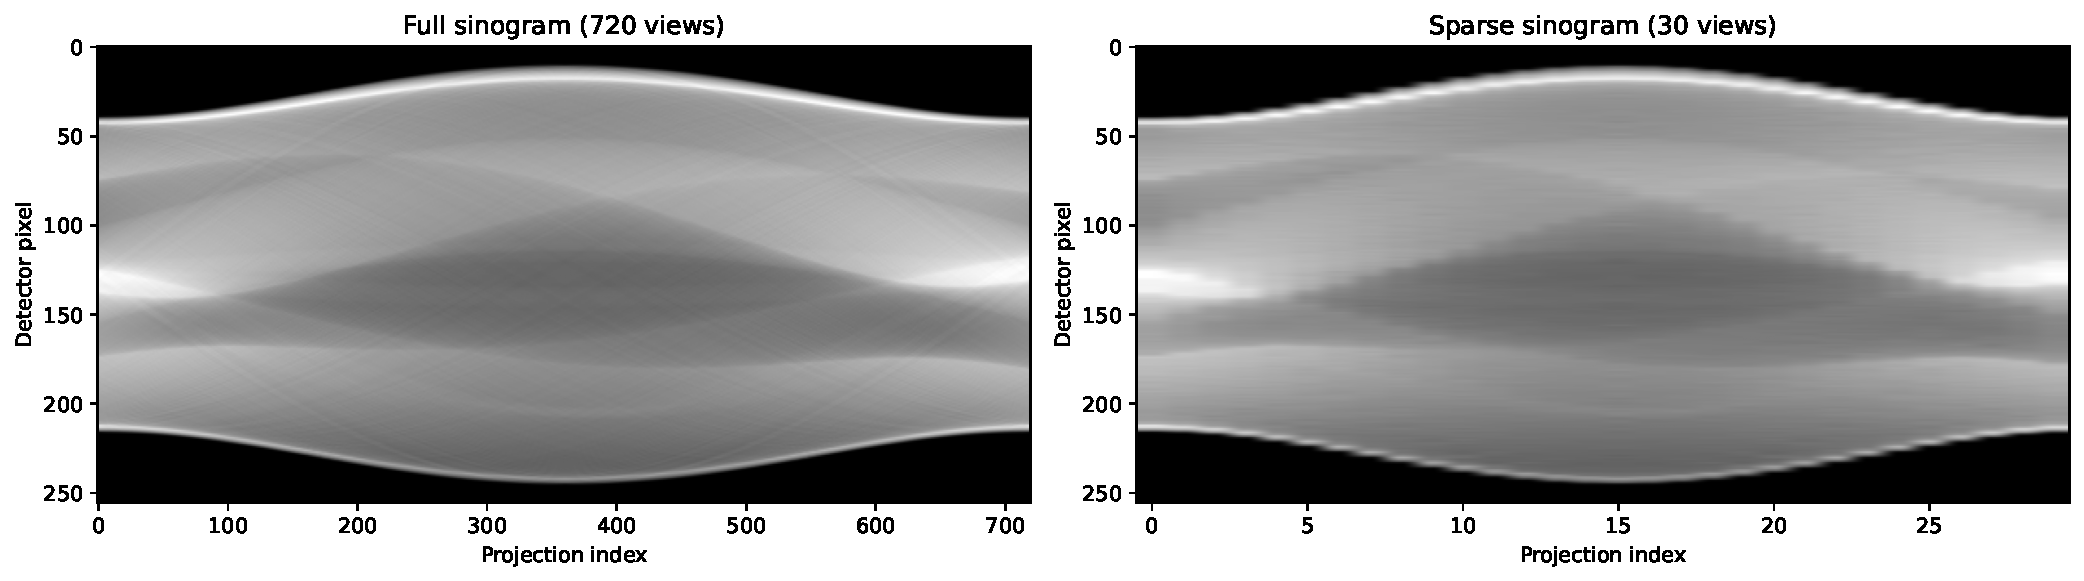
\includegraphics[width=\textwidth]{figures/sinogram_comparison.pdf}
    \caption{Sinogram comparison for the Shepp-Logan phantom. \textbf{Left}: full sinogram
             with 720 projection angles (the clinical standard). \textbf{Right}: sparse
             sinogram with only 30 angles, corresponding to a $24\times$ dosage reduction.
             The sparse sinogram contains the same sinusoidal structure but sampled at
             far fewer angular positions, leaving large gaps in the Radon domain.}
    \label{fig:sinogram-comparison}
\end{figure}

% -----------------------------------------------------------
\section{Ill-Posedness of the CT Inverse Problem}
\label{sec:ill-posedness}
% -----------------------------------------------------------

Recovering $\bm{x}$ from $\bm{y}$ is an \emph{inverse problem}. When measurements are
complete and noise-free, the Radon transform is invertible (via the classical inversion
formula); however, practical CT acquisition violates both conditions, rendering the
problem ill-posed in the sense of Hadamard \citep{Hadamard1923}: solutions may not
exist, may not be unique, or may not depend continuously on the data.

\subsection{Sources of Ill-Posedness}

\paragraph{Sparse-view CT.}
To reduce patient radiation dose---the primary concern motivating this project---one
reduces the number of projection angles. The Mayo Clinic Low Dose CT Grand Challenge
dataset \citep{MayoClinic} provides a canonical low-dose benchmark. When the number of
angles drops below the Nyquist-like sampling criterion (informally: at least $(\pi/2)N$
views for an $N \times N$ image), the sinogram is severely undersampled. Analytically,
the null space of the undersampled $A$ is non-trivial: many images $\bm{x}$ yield the
same measurements $\bm{y}$, so the problem is underdetermined ($m \ll n$). The artefacts
produced by naive reconstruction are radially symmetric streak artefacts aligned with
the missing-angle directions.

\paragraph{Limited-angle CT.}
A related but distinct scenario arises when projections are available only over a
restricted angular range (e.g., $[0\degree, 120\degree]$). In tomosynthesis and some industrial
settings this is unavoidable due to geometry constraints. Here the null space of $A$
contains low-frequency components aligned with the missing angular sector, producing
characteristic directional blurring.

\paragraph{Noise amplification.}
Even with a full set of angles, the continuous Radon inversion formula amplifies
high-frequency noise: it involves differentiation (the ramp filter in FBP), which
multiplies Fourier coefficients by $|\xi|$, the spatial frequency. Consequently, white
measurement noise $\bm{\eta}$ leads to high-frequency artefacts in naively inverted
images. Physically, quantum (Poisson) noise in the photon counts is the dominant
source \citep{Buzug2008}.

\paragraph{Formal characterisation.}
The singular value decomposition (SVD) of $A$ reveals the mechanism: the singular
values $\sigma_i$ of $A$ decay, often rapidly, towards zero. Inverting $A$ via
$\bm{x} = A^+ \bm{y}$ (the pseudoinverse) amplifies the components of $\bm{y}$ lying in the
direction of small singular vectors by $1/\sigma_i$, which diverges as
$\sigma_i \to 0$. This is the hallmark of a \emph{discrete ill-posed problem}
\citep{Hansen1992,Hansen1998}.

\begin{figure}[htbp]
    \centering
    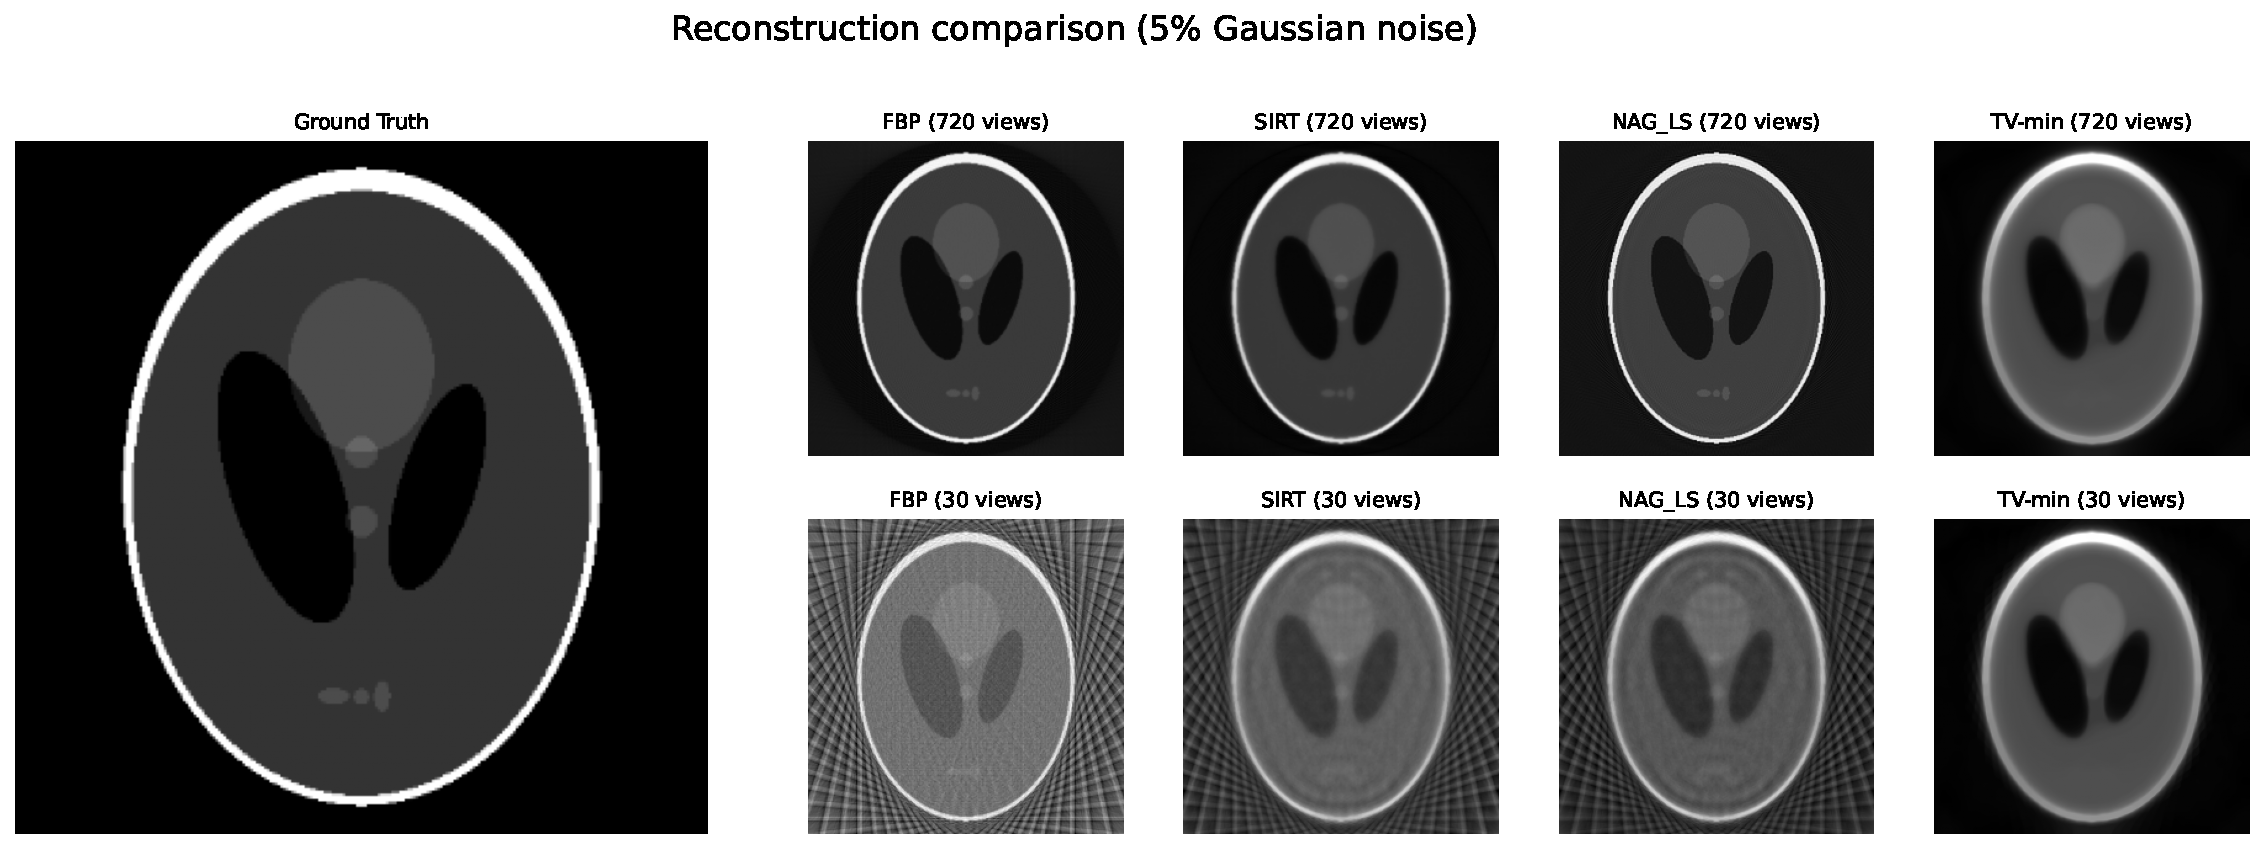
\includegraphics[width=\textwidth]{figures/reconstruction_comparison.pdf}
    \caption{Reconstruction comparison on the Shepp-Logan phantom with 5\% Gaussian noise.
             \textbf{Top row}: ground truth, FBP from 720 views (clinical reference), and
             FBP from 30 views (severe streak artefacts). \textbf{Bottom row}: SIRT, NAG\_LS,
             and TV minimisation, all from 30 views. The degradation from 720 to 30 views
             in FBP illustrates the ill-posedness of the sparse-view problem.}
    \label{fig:reconstruction-comparison}
\end{figure}

\subsection{Noise Model}

The physical acquisition process introduces Poisson-distributed noise in the photon
counts. After the log-transformation \eqref{eq:line-integral}, the sinogram noise is
approximately Gaussian for moderate dose levels (by the central limit theorem) and
can be written:
\begin{equation}
    \bm{\eta} \sim \mathcal{N}(\bm{0}, \sigma^2 I),
\end{equation}
where $\sigma^2$ depends on dose level. In the sparse-view CT experiments of the TFPnP
paper \citep{Wei2022TFPnP}, Gaussian noise with levels $\sigma \in \{5\%, 7.5\%, 10\%\}$
is added to the projections after the Radon transform, simulating realistic low-dose
acquisition at a $24\times$ dosage reduction compared to the 720-view standard.


% -----------------------------------------------------------
\section{Classical Reconstruction Algorithms}
\label{sec:classical-reconstruction}
% -----------------------------------------------------------

Before learned methods, three families of algorithms dominated CT reconstruction.
These serve as baselines in the experimental evaluation and underpin the learned methods
reviewed in \cref{chap:related-work}.

\subsection{Filtered Backprojection (FBP)}

Filtered backprojection is the standard clinical workhorse, derived analytically from the
inversion of the continuous Radon transform via the Central Slice Theorem. The algorithm
proceeds in two stages:

\begin{enumerate}
    \item \textbf{Filtering.} Each projection $p(\phi, \cdot)$ is convolved in the $s$-domain
          with a \emph{ramp filter} $h(s)$ whose Fourier transform is $|\xi|$, compensating
          for the non-uniform density of Fourier samples:
          \[
              \tilde{p}(\phi, s) = \bigl(p(\phi, \cdot) * h\bigr)(s).
          \]
    \item \textbf{Backprojection.} The filtered projections are smeared back into image space
          by integrating over all angles:
          \[
              f(\bm{x}) = \int_0^{\pi} \tilde{p}\!\left(\phi,\, \bm{x}\cdot\bm{\theta}\right)\mathrm{d}\phi.
          \]
\end{enumerate}

FBP is exact in the limit of dense, noiseless, full-angle sampling. Its principal
shortcomings are: (i) the ramp filter amplifies high-frequency measurement noise,
requiring an apodisation window (e.g., Hann, Ram-Lak) that blurs fine structures;
(ii) streak artefacts appear under sparse-view sampling. For cone-beam geometry, the
Feldkamp--Davis--Kress (FDK) algorithm \citep{Feldkamp1984} extends FBP and is
available in LION as \texttt{fdk}.

\subsection{Simultaneous Iterative Reconstruction Technique (SIRT)}

Iterative algebraic methods treat reconstruction as a least-squares problem:
\begin{equation}
    \min_{\bm{x}} \frac{1}{2}\|\,A\bm{x} - \bm{y}\,\|_2^2.
    \label{eq:least-squares}
\end{equation}
SIRT \citep{Gilbert1972} approximates the solution via gradient descent with a scaled step:
\begin{equation}
    \bm{x}^{(k+1)} = \bm{x}^{(k)} + C A^T R\!\left(\bm{y} - A\bm{x}^{(k)}\right),
\end{equation}
where $C = \operatorname{diag}(1/\sum_i A_{ij})$ and $R = \operatorname{diag}(1/\sum_j A_{ij})$
are diagonal scaling matrices (column and row sums of $A$) that normalise the step and
ensure convergence. SIRT converges to the minimum $\ell^2$-norm least-squares solution.
It handles missing data more gracefully than FBP (no explicit ramp amplification), but
converges slowly and is still unstable in the presence of noise without early stopping or
regularisation. LION provides a differentiable implementation via
\texttt{ts\_algorithms.SIRT}.

\subsection{Total Variation Minimisation}

Motivated by the observation that medical CT images are approximately piecewise constant
(and thus have sparse gradients), \citet{RudinOsherFatemi1992} introduced the
\emph{total variation} (TV) regulariser:
\begin{equation}
    \mathrm{TV}(\bm{x}) = \|\nabla \bm{x}\|_1
        = \sum_{i,j} \sqrt{|\partial_x x_{ij}|^2 + |\partial_y x_{ij}|^2},
\end{equation}
and \citet{SidkyPan2008} applied it to CT reconstruction as:
\begin{equation}
    \min_{\bm{x} \geq 0}\;\mathrm{TV}(\bm{x})
        \quad \text{subject to} \quad \|A\bm{x} - \bm{y}\|_2 \leq \varepsilon,
    \label{eq:tv-min}
\end{equation}
where $\varepsilon$ bounds the noise level. This is a convex optimisation problem solvable
by primal-dual splitting methods, such as the Primal-Dual Hybrid Gradient (PDHG) algorithm
of \citet{ChambolleAndPock2011}, available in LION as \texttt{tv\_min}. TV
reconstruction produces visually clean images with preserved edges, but can introduce
the characteristic \emph{staircase artefact} and requires careful selection of $\lambda$
(or equivalently $\varepsilon$). In the TFPnP sparse-view CT experiments, TV with
optimally tuned parameters achieves 20.91/19.17/16.95\,dB PSNR for the three noise
levels---substantially above FBP but below learned methods \citep{Wei2022TFPnP}.

\begin{figure}[htbp]
    \centering
    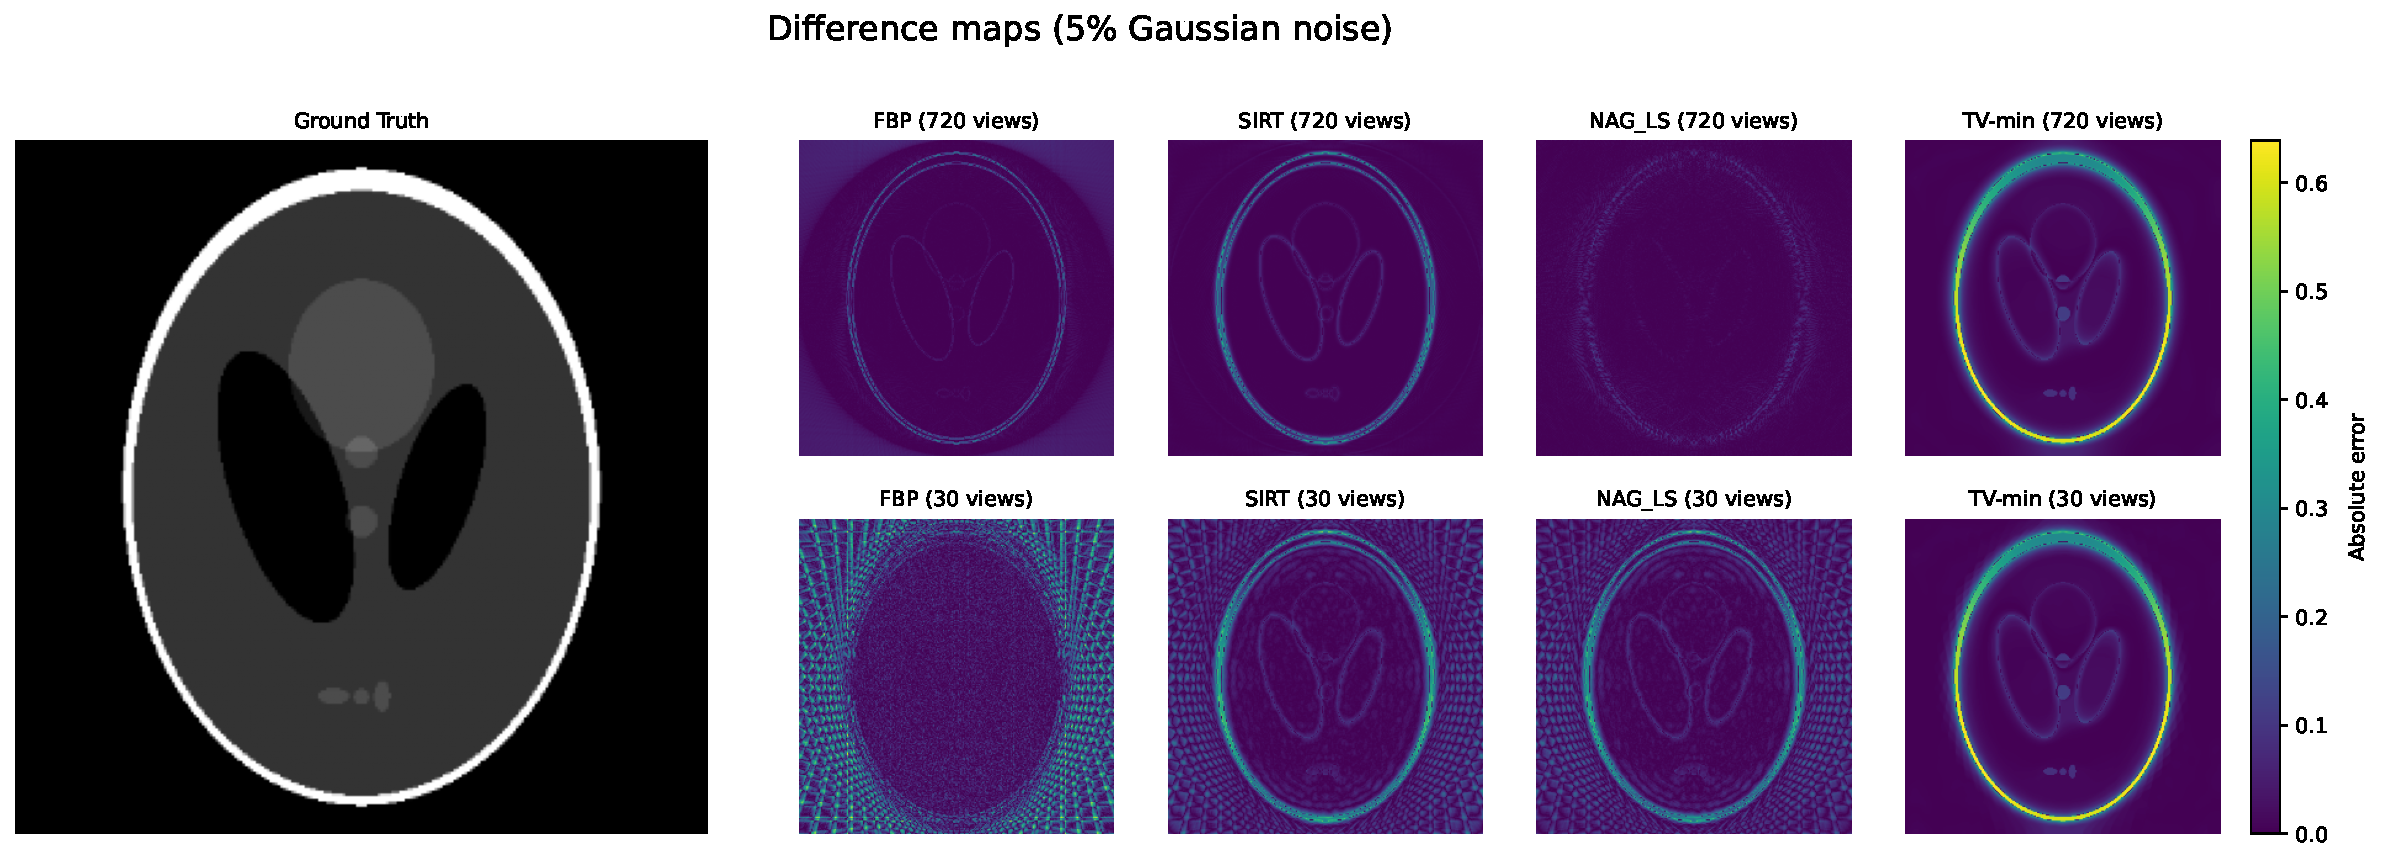
\includegraphics[width=\textwidth]{figures/difference_maps.pdf}
    \caption{Difference maps $\hat{\bm{x}} - \bm{x}^*$ for three reconstruction methods
             from 30-view sparse sinograms with 5\% noise. \textbf{Left}: FBP shows
             structured streak artefacts (correlated error). \textbf{Centre}: SIRT shows
             diffuse error concentrated at edges. \textbf{Right}: TV minimisation achieves
             the lowest error overall but shows sharp transitions at edges characteristic
             of the staircase artefact.}
    \label{fig:difference-maps}
\end{figure}

\subsection{From Classical to Learned: A Bridge}
\label{sec:bridge}

The fundamental limitation of both FBP and iterative methods is that they either
(a) invert the forward model analytically without data-driven priors (FBP), or
(b) assume a hand-crafted regulariser such as TV whose inductive bias may not align with
the true distribution of CT images. The key question motivating the field of learned
reconstruction is: \emph{can we replace or supplement the hand-crafted prior with one
learned directly from data?} \Cref{chap:related-work} surveys the spectrum of approaches
that have emerged to address this question---from variational regularisation through deep
unrolling to plug-and-play methods---culminating in TFPnP, the method implemented in
this project.

% ==============================================================================
% Chapter 3: Design and Implementation
% ==============================================================================
% ============================================================
%  Chapter 3: Design and Implementation
% ============================================================

\chapter{Design and Implementation}
\label{chap:implementation}

% ============================================================
%  Section 3.1 — Overview of the pipeline
% ============================================================
\section{Overview}
\label{sec:overview}

The reproduction is implemented as a Python package, \texttt{ct\_tfpnp}, that integrates with the LION toolbox~\citep{Biguri2024LION} for the CT geometry, forward operator, and dataset handling. The package contains
all the components of the TFPnP algorithm, including the ResNet-18 policy network, the residual value network, the ADMM environment, the DRUNet denoiser wrapper, and the RL training loop, as well as the baseline reconstruction methods (FBP, TV, DRUNet alone, FBPConvNet, and Fixed PnP-ADMM) used for comparison.

The full experimental pipeline covers eleven trained TFPnP runs and two baseline model checkpoints (FBPConvNet and a CT-trained DRUNet), with each run producing a set of diagnostic figures via \texttt{scripts/evaluate\_run.py}, including training curves, per-image metrics, policy behaviour, and a reconstruction gallery. All experiments are launched on the Cambridge Service for Data Driven
Discovery (CSD3) HPC cluster through SLURM job scripts (see~\Cref{app:supplementary}), with outputs written to a results directory for analysis.

% ============================================================
%  Section 3.2 — Geometry, data, and noise conventions
% ============================================================
\section{Geometry, data, and noise conventions}
\label{sec:geometry-noise}

All experiments use a sparse 30-view parallel-beam geometry, matching~\citet{Wei2022TFPnP}. As LION had no matching preset, a custom \texttt{Geometry} object was constructed with 30 angles uniformly spaced over $[0, \pi)$, a $512 \times 512$ image, and 724 detectors ($[512\sqrt{2}]$, chosen to cover the image diagonal). The forward operator is LION's \texttt{CTProjectionOp}, a thin wrapper around tomosipo~\citep{Hendriksen2021Tomosipo}, whereas \citet{Wei2022TFPnP} use TorchRadon~\citep{Ronchetti2020TorchRadon}. The two are mathematically equivalent but differ in scaling conventions (\Cref{sec:admm-gradient}).

Training and evaluation data come from LIDC-IDRI~\citep{Armato2011LIDC}, split at the patient level into 80/10/10 partitions using LION's default loader. This yields approximately 3300, 401, and 389 slices in the training, validation, and test splits respectively, with up to 5 slices per patient and a 50/50 nodule-to-non-nodule ratio. \citet{Wei2022TFPnP} evaluate on 50 randomly selected lung slices from the COVID-19 CT lung and infection segmentation dataset~\citep{Ma2020COVID19}, making our test set substantially larger. \Cref{fig:sample_lidc} shows a representative training slice.

Image intensities are preserved in linear attenuation coefficient ($\mu$) units throughout the pipeline, with values approximately in $[0, 2.5]$\,cm$^{-1}$. This convention is set by LION's LIDC loader via its \texttt{from\_HU\_to\_mu} transform, and is preserved rather than rescaled to $[0, 1]$ as in many other reproductions, to retain the physical interpretation of reconstructed values.

Sinogram noise is added following~\citet{Wei2022TFPnP}'s percentage-of-signal-standard-deviation convention. For each ground truth image, the clean sinogram $y_{\text{clean}} = Ax_{\text{gt}}$ is normalised by a per-image factor $\text{SCALE} = y_{\text{clean}}.\text{max}() / x_{\text{gt}}.\text{max}()$ so that the percentage noise fraction applies consistently across images. Additive Gaussian noise is then applied at 5\%, 7.5\%, or 10\% of the normalised sinogram's standard deviation, and the result is rescaled back to the original operator range. Noise seeds are deterministic per image (\texttt{seed = img\_idx * 100}), so paired comparisons between methods use identical realisations.

LION provides a more physically realistic \texttt{sinogram\_add\_noise} routine based on a Poisson-Gaussian model, which would better represent the photon-counting statistics of real CT acquisitions, but it takes physical parameters (photon count, detector gain) rather than a percentage noise fraction, so its noise levels do not map directly onto the paper's 5\%, 7.5\%, 10\% conditions. The paper's percentage convention is used here to keep the implementation as close to~\citet{Wei2022TFPnP}'s as possible and preserve the direct comparability of results.

One consequence of retaining native $\mu$ units is that PSNR values in this report are approximately $5$\,dB higher than those reported in~\citet{Wei2022TFPnP}, affecting cross-study comparisons but not within-experiment rankings (\Cref{sec:metrics}).

% ------------------------------------------------------------
%  Figure 3.1: Sample training image (lung slice) from LIDC
% ------------------------------------------------------------
\begin{figure}[H]
    \centering
    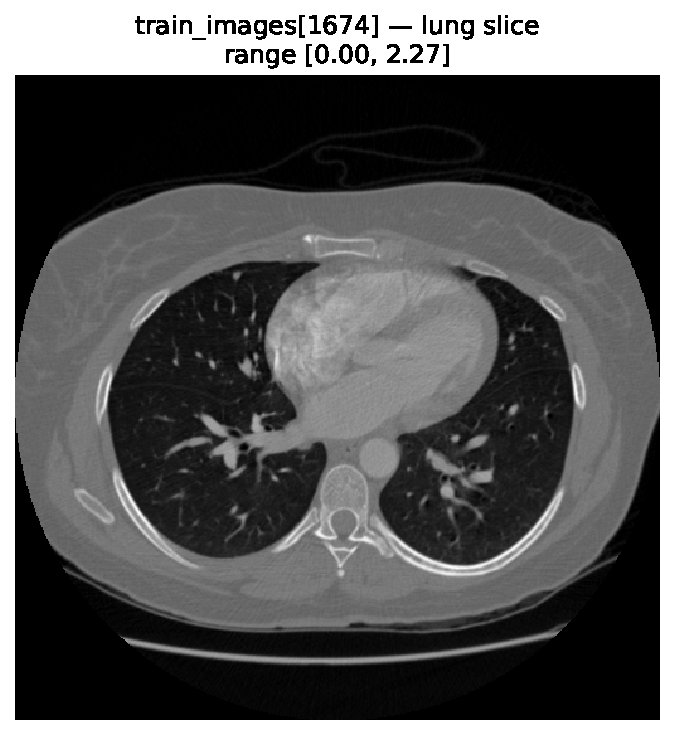
\includegraphics[width=0.5\linewidth]{../figures/12/01_sample_train_image.pdf}
    \caption{A lung slice from the LIDC-IDRI training split, in native $\mu$ units (approximately $[0,2.3]$\,cm$^{-1}$).}
    \label{fig:sample_lidc}
\end{figure}

% ============================================================
%  Section 3.3 — TFPnP policy and RL training
% ============================================================
\section{TFPnP policy and RL training}
\label{sec:tfpnp-policy}

The TFPnP policy network follows the architecture described by~\citet{Wei2022TFPnP}. A ResNet-18 backbone extracts features from a five-channel input consisting of the current ADMM iterates $(x, z, u)$, a noise-level map, and an iteration-progress map. Two output heads share the resulting 512-dimensional feature vector, a two-way termination head predicting whether to stop, and a parameter head predicting the next $m = 5$ pairs of $(\sigma, \mu)$ via a sigmoid activation rescaled to the configured action ranges.

The backbone follows torchvision's ResNet-18, with only the first convolutional layer replaced to accept five input channels rather than three. Table~1 of~\citet{Wei2022TFPnP} specifies a $3 \times 3$ stem, whereas torchvision's default is $7 \times 7$, which is retained for this implementation. Our slices are $512 \times 512$, so layer4 emits $16 \times 16$ rather than $4 \times 4$, but an adaptive average pool absorbs the difference. Both deviations are recorded in~\Cref{tab:implementation-differences}.

Table~1 gives conv1 an output of $64 \times 64$ and layer1 an output of $32 \times 32$, but does not state how this is obtained, since a standard ResNet-18's layer1 does not downsample. We retain torchvision's max-pooling layer, which reproduces the stated output sizes.

The value network departs from the paper. The caption of Table~1 specifies the same feature extractor as the policy, with batch normalisation replaced by weight normalisation and ReLU replaced by TReLU. Our value network is instead a residual network of eight blocks at constant width 64, with no normalisation, standard ReLU activations, no spatial downsampling, and a final linear layer mapping a 64-dimensional feature vector to the scalar value estimate. It preserves the paper's removal of batch normalisation but not the replacements specified alongside it. The consequences of this divergence are analysed in~\Cref{sec:in-domain-gap}.

Policy action ranges are $\sigma \in [1, 5]$ and $\mu \in [10, 100]$. The $\sigma$ range is calibrated to the natural-image DRUNet's useful operating region for CT, identified from a preliminary sensitivity sweep (\Cref{sec:calibration}) in which $\sigma > 5$ over-smoothed reconstructions. The $\mu$ range balances against the normalised data-fidelity gradient (\Cref{sec:admm-gradient}), with \citet{Wei2022TFPnP}'s corresponding effective range set at $[0.01, 1]$ because their unnormalised gradient is $\sim 100\times$ smaller.

The RL formulation matches~\citet{Wei2022TFPnP}'s equations 15--17. The value network is trained on a temporal-difference (TD) loss, which regresses each state's value estimate towards the reward received plus the discounted estimate of the next state, with discount factor $\gamma = 0.99$. Stability is maintained by comparing against a target network, a slowly-updated copy of the value network, refreshed by exponential moving average at rate $10^{-3}$. The termination policy $\pi_1$ uses a value baseline, subtracting the value network's prediction from the reward before applying the REINFORCE update, which reduces gradient variance. The reward is $r = \Delta\text{PSNR} - \eta$ with $\eta = 0.05$.

Learning rates are $10^{-4}$ for the critic, $3 \times 10^{-5}$ for the shared policy features and termination head, and $10^{-6}$ for the parameter head, the last kept low to compensate for the sensitivity of $\pi_2$'s gradient through the ADMM rollout. The paper's hyperparameters $m = 5$, $N = 6$, and $\eta = 0.05$ are preserved exactly.

% ============================================================
%  Section 3.4 — ADMM step and z-step gradient normalisation
% ============================================================
\section{ADMM step and z-step gradient normalisation}
\label{sec:admm-gradient}

The ADMM environment implements~\citet{Wei2022TFPnP}'s equations 7--9, with each outer iteration performing three sub-steps. The $x$-step applies the DRUNet denoiser as an implicit image prior, the $z$-step enforces data fidelity against the noisy sinogram, and the $u$-step updates the dual variable to accumulate constraint violation.

The $z$-step is solved by six iterations of gradient descent, so that the update is differentiable end-to-end. The model-based DDPG update for $\pi_2$ requires backpropagation through the entire $z$-step, which gradient descent supports through automatic differentiation.

LION's adjoint operator $A^{\top}$ implements the raw backprojection of tomosipo's discrete Radon transform, summing sinogram values along ray paths without normalisation, so $A^{\top}(Az)$ produces per-voxel values much larger than the input image. Without adjustment, the data-fidelity gradient $A^{\top}(Az - y)$ would dominate the proximal term $\mu(z - \text{target})$ for any reasonable $\mu$, rendering the policy's $\mu$ predictions meaningless. To resolve this, the backprojected residual is normalised to unit maximum before being combined with the proximal term,

\begin{equation}
\text{grad} = \frac{A^{\top}r}{\|A^{\top}r\|_\infty + \epsilon} +
              \mu(z - \text{target}),
\end{equation}

where $r = Az - y$ is the sinogram residual and $\epsilon = 10^{-8}$ prevents division by zero. The proximal term pulls $z$ towards the current ADMM estimate $\text{target} = x + u$, with $\mu$ controlling the strength. Normalising the first term places its magnitude on the same scale as the proximal term, so $\mu$ can meaningfully balance the two. The gradient step size is further scaled as $\alpha / (1 + \mu)$, with $\alpha = 1$, to keep the update bounded as $\mu$ grows. Our absolute $\mu$ values therefore differ from~\citet{Wei2022TFPnP}'s in scale but preserve their role in the ADMM balance, as reflected in the $\mu \in [10, 100]$ action range (\Cref{sec:tfpnp-policy}).

% ============================================================
%  Section 3.5 — Baselines
% ============================================================
\section{Baselines}
\label{sec:baselines}

The TFPnP reproduction is validated against five baseline methods. Three of the paper's baselines (RED-CNN, LPD, RPGD) are either absent from LION or would require training beyond the project timeline, so were not included.

\textbf{FBP} applies a Ram-Lak filter followed by unfiltered backprojection through LION's operator, with the analytical normalisation $\pi / (2N)$ for $N = 30$ projection angles. The result is clamped to non-negative values.

\textbf{TV reconstruction} uses ISTA with 200 iterations and anisotropic total variation at regularisation strength $\lambda = 0.01$. The data-fidelity gradient is normalised to unit maximum before each step, matching the ADMM z-step convention (\Cref{sec:admm-gradient}), and non-negativity is enforced after each iteration.

\textbf{DRUNet alone} applies the natural-image DRUNet as a single denoising pass over the FBP reconstruction, with fixed $\sigma = 10$. This is not one of~\citet{Wei2022TFPnP}'s baselines, but provides a useful lower bound, isolating how much of TFPnP's performance comes from ADMM's iterative refinement rather than the denoiser itself.

\textbf{FBPConvNet}~\citep{Jin2017FBPConvNet} is a five-stage U-Net mapping sparse-view FBP reconstructions to full-view ground truth. Our FBPConvNet is trained end-to-end on the LIDC training split (250 patients across 80 epochs) using LION's implementation, with MSE loss and Adam at learning rate $10^{-4}$, at a fixed 5\% sinogram noise level. This departs both from~\citet{Jin2017FBPConvNet}'s original protocol (clean projections at training, noise added at inference) and from~\citet{Wei2022TFPnP}'s FBPconv, whose near-constant PSNRs across noise levels (23.00, 22.94, 22.86\,dB) implies mixed-noise training, although this is not explicitly stated. Fixed 5\% training makes evaluation at 7.5\% and 10\% out-of-distribution, and is central to the reversal narrative in~\Cref{sec:headline}.

\textbf{Fixed PnP-ADMM} uses the same ADMM environment as TFPnP with hand-calibrated $\sigma = 1.5$ and $\mu = 20$, selected as the operating point maximising PSNR on a preliminary sweep. Any improvement of TFPnP over Fixed PnP-ADMM can be attributed to policy-based hyperparameter adaptation.

% ============================================================
%  Section 3.6 — CT-specific DRUNet training
% ============================================================
\section{CT-specific DRUNet training}
\label{sec:ct-drunet}

The headline TFPnP result (\texttt{run\_04}) uses the natural-image DRUNet as denoiser prior, matching~\citet{Wei2022TFPnP}. As an extension, a CT-specific DRUNet is trained to test whether an in-domain denoiser improves reconstruction quality. The same architecture and checkpoint format as the pretrained natural-image DRUNet~\citep{zhang2021plug} is used, making it a drop-in replacement.

Training uses the LIDC training split (3300 slices) for 50 epochs with Adam at learning rate $10^{-4}$, a cosine annealing schedule, and batch size 8. Each mini-batch samples a random noise level $\sigma \in [0, 50]$ per image, following~\citet{zhang2021plug}'s multi-level convention, and loss is computed using mean squared error in the per-image $[0, 1]$ normalised space to match the DRUNet's input convention. Validation PSNR at $\sigma \in \{5, 15, 25\}$ is monitored throughout training, with best-checkpoint selection based on PSNR at $\sigma = 15$. \Cref{fig:ct_drunet_training} shows the training progression.

An initial drop-in test using the CT-DRUNet in place of the natural-image DRUNet within \texttt{run\_04}'s TFPnP pipeline revealed a calibration mismatch, with PSNR collapsing to approximately $13$\,dB, below the FBP baseline. Diagnosis showed that the CT-DRUNet's optimal $\sigma$ sits at approximately $8$, indicating that
the regularisation scale at which the denoiser is most useful shifts with the training data distribution. When each denoiser is compared at its calibrated optimum, the CT-DRUNet outperforms the natural-image DRUNet at every noise level, with an advantage that grows with noise (\Cref{sec:in-domain}).

% ------------------------------------------------------------
%  Figure 3.3: CT-DRUNet training curves
% ------------------------------------------------------------
\begin{figure}[H]
    \centering
    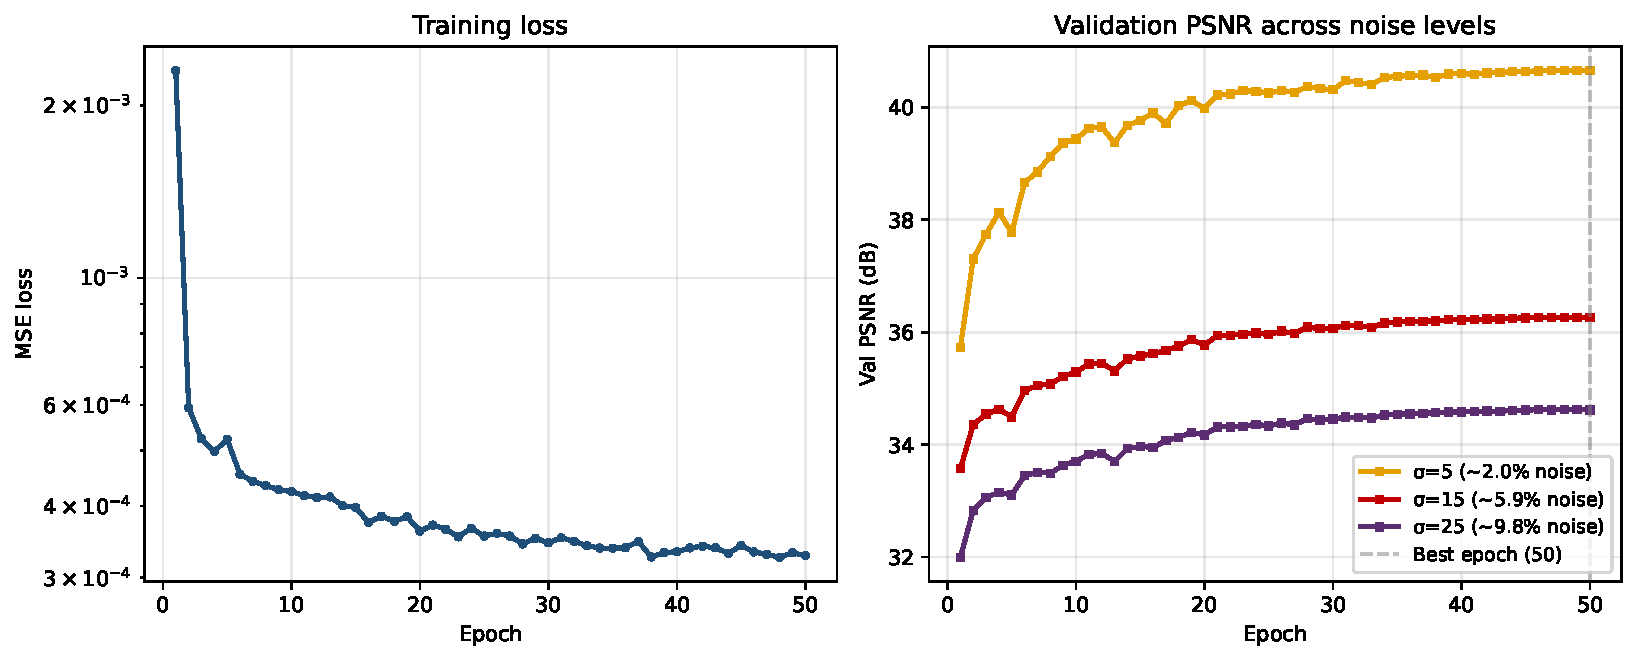
\includegraphics[width=\linewidth]{../figures/12/04_full_training_curves.pdf}
    \caption{CT-DRUNet training curves. Left, MSE loss on the LIDC
    training split over 50 epochs. Right, validation PSNR at
    $\sigma \in \{5, 15, 25\}$. Best checkpoint selected by peak
    validation PSNR at $\sigma = 15$.}
    \label{fig:ct_drunet_training}
\end{figure}

% ============================================================
%  Section 3.7 — Compute infrastructure
% ============================================================
\section{Compute infrastructure}
\label{sec:compute}

All experiments were run on the Cambridge Service for Data Driven Discovery (CSD3) HPC cluster, using GPUs on the \texttt{ampere} partition. GPU access was allocated through a single account, \texttt{MPHIL-DIS-SL2-GPU}, which limited the number of ablation runs and rescue attempts feasible within the project timeline. All jobs were managed through SLURM, with a project-specific conda environment (\texttt{mphil\_ct}) providing the LION toolbox, PyTorch, tomosipo, and supporting packages.

% ============================================================
%  Section 3.8 — Summary of implementation differences from Wei et al.
% ============================================================
\begin{table}[H]
    \centering
    \footnotesize
    \caption{Implementation choices differing from \citet{Wei2022TFPnP}.}
    \label{tab:implementation-differences}
    \begin{tabular}{L{3.5cm}L{3cm}L{3cm}L{4cm}}
        \toprule
        Aspect                & \citet{Wei2022TFPnP} & Ours & Reason \\
        \midrule
        CT geometry            & 30-view TorchRadon        & 30-view custom LION \texttt{Geometry}  & LION had no matching preset \\ \hline
        Detector count         & 182                       & 724 ($\lceil 512\sqrt{2}\,\rceil$) & Cover image diagonal without truncation \\ \hline
        Forward projector      & TorchRadon                & LION + tomosipo & LION native \\ \hline
        Policy backbone stem   & $3\times3$                & $7\times7$ (torchvision default) & Stage widths and $/32$ downsampling unchanged; retraining to match was outside the compute budget \\ \hline
        Value network          & Policy feature extractor with weight norm + TReLU & Eight residual blocks at width 64, no normalisation, standard ReLU & Simpler BN-free critic \\ \hline
        Policy input resolution & $128\times128$           & $512\times512$ native slice & ADMM state passed at full resolution \\ \hline
        Image intensity scale  & [0, 1] normalized         & Native $\mu$ & Preserve physical units \\ \hline
        z-step gradient norm   & None                      & Normalized $A^{\top}r$ & Compensate LION operator scaling \\ \hline
        PSNR data range        & Not stated (likely 1.0)   & Per-image $x_{\text{gt}}.\text{max}()$ & Matches~\texttt{data\_range} in LION conventions \\ \hline
        PSNR / SSIM backend    & Not specified             & Custom PyTorch reimplementations of LION reference & Differentiability for ADMM step \\ \hline
        HaarPSI backend        & Not used                  & \texttt{piq} library & Compatible with $\mu$-unit inputs \\ \hline
        Policy $\sigma$ range  & Not stated                & $[1, 5]$ & Calibration for natural DRUNet \\ \hline
        Policy $\mu$ range     & Not stated                & $[10, 100]$ & Effective range post-gradient-normalization \\ \hline
        Denoiser training data & BSD400 natural images     & Same (\texttt{run\_04}) LIDC (\texttt{run\_11}) & In-domain extension \\ \hline
        Denoiser $\sigma$ range & $[1, 50]$                & $[0, 50]$ (\texttt{run\_11}) & Following~\citet{zhang2021plug} \\ \hline
        Denoiser loss          & $L_1$                     & MSE  & Simpler default, PSNR-aligned \\ \hline
        Denoiser batch size    & 32                        & 8    & Fits GPU budget \\ \hline
        Policy learning rates  & $l_\theta{=}10^{-4}$, $l_\phi{=}5{\times}10^{-5}$ (later halved) & Critic $10^{-4}$, policy $3{\times}10^{-5}$, param $10^{-6}$ & Empirical stability with our action ranges \\ \hline
        Policy training data   & PASCAL VOC natural images & LIDC (all runs) & In-domain policy training \\ \hline
        FBPConvNet training noise & Mixed (implied by flat PSNR) & 5\% fixed & Simplest testable regime \\ \hline
        Test set               & COVID-19 lung, 50 images  & LIDC-IDRI, 389 images & LION-native dataset \\
        \bottomrule
    \end{tabular}
\end{table}

% ============================================================
%  Section 3.9 — Evaluation metrics
% ============================================================
\section{Evaluation metrics}
\label{sec:metrics}
Reconstruction quality is evaluated using peak signal-to-noise ratio (PSNR)~\citep{Wang2004SSIM}, structural similarity index (SSIM)~\citep{Wang2004SSIM}, and Haar wavelet-based perceptual similarity index (HaarPSI)~\citep{Reisenhofer2018HaarPSI}. PSNR is the standard metric used by~\citet{Wei2022TFPnP} and is essential for direct comparison to their reported results. The motivation for reporting SSIM and HaarPSI alongside PSNR is discussed in~\Cref{sec:metrics-discussion}.

PSNR and SSIM are reimplemented in PyTorch to preserve differentiability through the reward computation chain, which is required for the model-based $\pi_2$ policy gradient's backpropagation through the ADMM environment. Both reimplementations follow LION's per-image convention using \texttt{data\_range}$= x_{\text{gt}}.\text{max}()$. HaarPSI is used only at evaluation time, so no custom implementation is required, allowing it to be loaded from the \texttt{piq} library~\citep{Kastryulin2022PIQ}, which accepts a configurable \texttt{data\_range} compatible with our $\mu$-scaled inputs. LION's own HaarPSI implementation requires inputs strictly in $[0, 1]$ and was not used to avoid per-image normalisation. All metrics are computed per-image and averaged over the test set.

% ============================================================
%  Section 3.10 — Reproducibility difficulties
% ============================================================
\section{Reproducibility difficulties}
\label{sec:reproducibility-difficulties}

Several aspects of~\citet{Wei2022TFPnP}'s methodology were ambiguous or underspecified, requiring interpretation during reproduction. The paper does not explicitly state the PSNR data range convention, the baseline TV solver, the FBPconv training regime, or the ADMM $z$-step solver used for CT. The choices made in each case are documented in~\Cref{tab:implementation-differences}.

\textbf{Reference code differences.} The paper's forward operator uses TorchRadon~\citep{Ronchetti2020TorchRadon}, which returns sinograms already scaled by the ray-length correction. LION's tomosipo-based operator does not apply this correction, propagating the mismatch through the pipeline and requiring FBP normalisation, ADMM gradient scaling (the $\mu$ range), and the SCALE factor in noise generation (\Cref{sec:geometry-noise}).

\textbf{RL training stability.} When the $\sigma$ range was widened from $[1, 5]$ to $[1, 15]$ to accommodate the CT-trained DRUNet in \texttt{run\_11}, the critic loss exploded around policy update step 15{,}000 and the policy $\sigma$ output collapsed (\Cref{sec:run11}). Our value network is not the one specified in Table~1 of~\citet{Wei2022TFPnP}, so this instability cannot be attributed to the paper's formulation. Stabilising RL training with widened action ranges under our critic requires careful hyperparameter tuning (\Cref{sec:in-domain-gap}).

\textbf{What worked well.} \citet{Wei2022TFPnP}'s reward function ($r = \Delta\text{PSNR} - \eta$), MDP formulation, and Algorithm~1 were sufficiently clear to reproduce directly, and the two-network policy--value architecture is straightforward to implement. The reproduction follows the paper's algorithm closely and produces results within the paper's reported range, subject to the architectural deviations recorded in~\Cref{tab:implementation-differences}.

% ==============================================================================
% Chapter 4: Evaluation
% ==============================================================================
% ============================================================
%  Chapter 4: Evaluation
% ============================================================

\chapter{Evaluation}
\label{chap:results}

% ============================================================
%  Section 4.1 — Headline reproduction result
% ============================================================
\section{Headline reproduction result}
\label{sec:headline}

The headline TFPnP result comes from \texttt{run\_04\_pat\_250\_e80}, where the policy is trained on 250 LIDC patients over 80 epochs, using the natural-image DRUNet as the denoiser prior and PSNR as the reward function. All evaluations use the full LIDC-IDRI test set (389 images) at three sinogram noise levels (5\%, 7.5\%, 10\%). The full experiment configuration is documented in~\Cref{sec:tfpnp-policy}.

Six reconstruction methods are compared, including classical baselines (FBP and TV), the denoiser applied directly to the FBP reconstruction (DRUNet), an end-to-end learned network (FBPConvNet), and two hyperparameters, and the TFPnP reproduction with the learned policy). \Cref{tab:headline_full} reports mean PSNR, SSIM, and HaarPSI at each noise level.

The reproduction confirms the paper's central claim, with TFPnP achieving \textbf{27.27\,dB} PSNR at 5\% noise, a $+2.96$\,dB improvement over Fixed PnP-ADMM. Perceptual metrics (SSIM $= 0.691$, HaarPSI $= 0.485$) improve similarly over Fixed PnP-ADMM ($0.499$ and $0.405$), confirming that the learned policy provides measurable value across all metrics.

One finding departs from the paper's ranking. FBPConvNet reaches $28.58$\,dB at 5\% noise, $+1.31$\,dB above TFPnP, whereas~\citet{Wei2022TFPnP} report TFPnP ahead of FBPconv by $+1.50$\,dB. The ranking inverts by 10\% noise (\Cref{sec:cross-noise}), and the underlying causes are analysed in~\Cref{sec:why-fbpconvnet}. \Cref{fig:reconstruction_gallery} shows a visual comparison of the best, median, and worst reconstructions.

% ------------------------------------------------------------
%  Table 4.1: Full test set × 3 noise levels × 6 methods × 3 metrics
% ------------------------------------------------------------
\begin{table}[H]
    \centering
    \footnotesize
    \caption{Reconstruction quality on the LIDC-IDRI test set (389 images).
    Best in \textbf{bold}, second-best \underline{underlined}.}
    \label{tab:headline_full}
    \begin{tabular}{lccc ccc ccc}
        \toprule
        & \multicolumn{3}{c}{\textbf{5\% noise}}
        & \multicolumn{3}{c}{\textbf{7.5\% noise}}
        & \multicolumn{3}{c}{\textbf{10\% noise}} \\
        \cmidrule(lr){2-4} \cmidrule(lr){5-7} \cmidrule(lr){8-10}
        Method & PSNR & SSIM & HaarPSI & PSNR & SSIM & HaarPSI & PSNR & SSIM & HaarPSI \\
        \midrule
        FBP                    & 14.56 & 0.075 & 0.233 & 13.65 & 0.058 & 0.223 & 13.22 & 0.052 & 0.216 \\
        TV                     & 19.67 & 0.288 & 0.390 & 18.35 & 0.271 & 0.348 & 17.50 & 0.248 & 0.315 \\
        DRUNet ($\sigma{=}10$) & 21.80 & 0.455 & 0.384 & 19.50 & 0.418 & 0.312 & 18.16 & 0.391 & 0.245 \\
        FBPConvNet             & \textbf{28.58} & \textbf{0.726} & \textbf{0.556} & \textbf{27.14} & 0.619 & \textbf{0.490} & 24.73 & 0.463 & 0.385 \\
        Fixed PnP-ADMM         & 24.31 & 0.499 & 0.405 & 22.42 & 0.376 & 0.336 & 21.50 & 0.340 & 0.290 \\
        TFPnP (Ours)           & \underline{27.27} & \underline{0.691} & \underline{0.485} & \underline{26.58} & \textbf{0.681} & \underline{0.443} & \textbf{26.10} & \textbf{0.676} & \textbf{0.413} \\
        \bottomrule
    \end{tabular}
\end{table}

% ------------------------------------------------------------
%  Figure 4.1: Contact-sheet reconstruction gallery
% ------------------------------------------------------------
\begin{figure}[H]
    \centering
    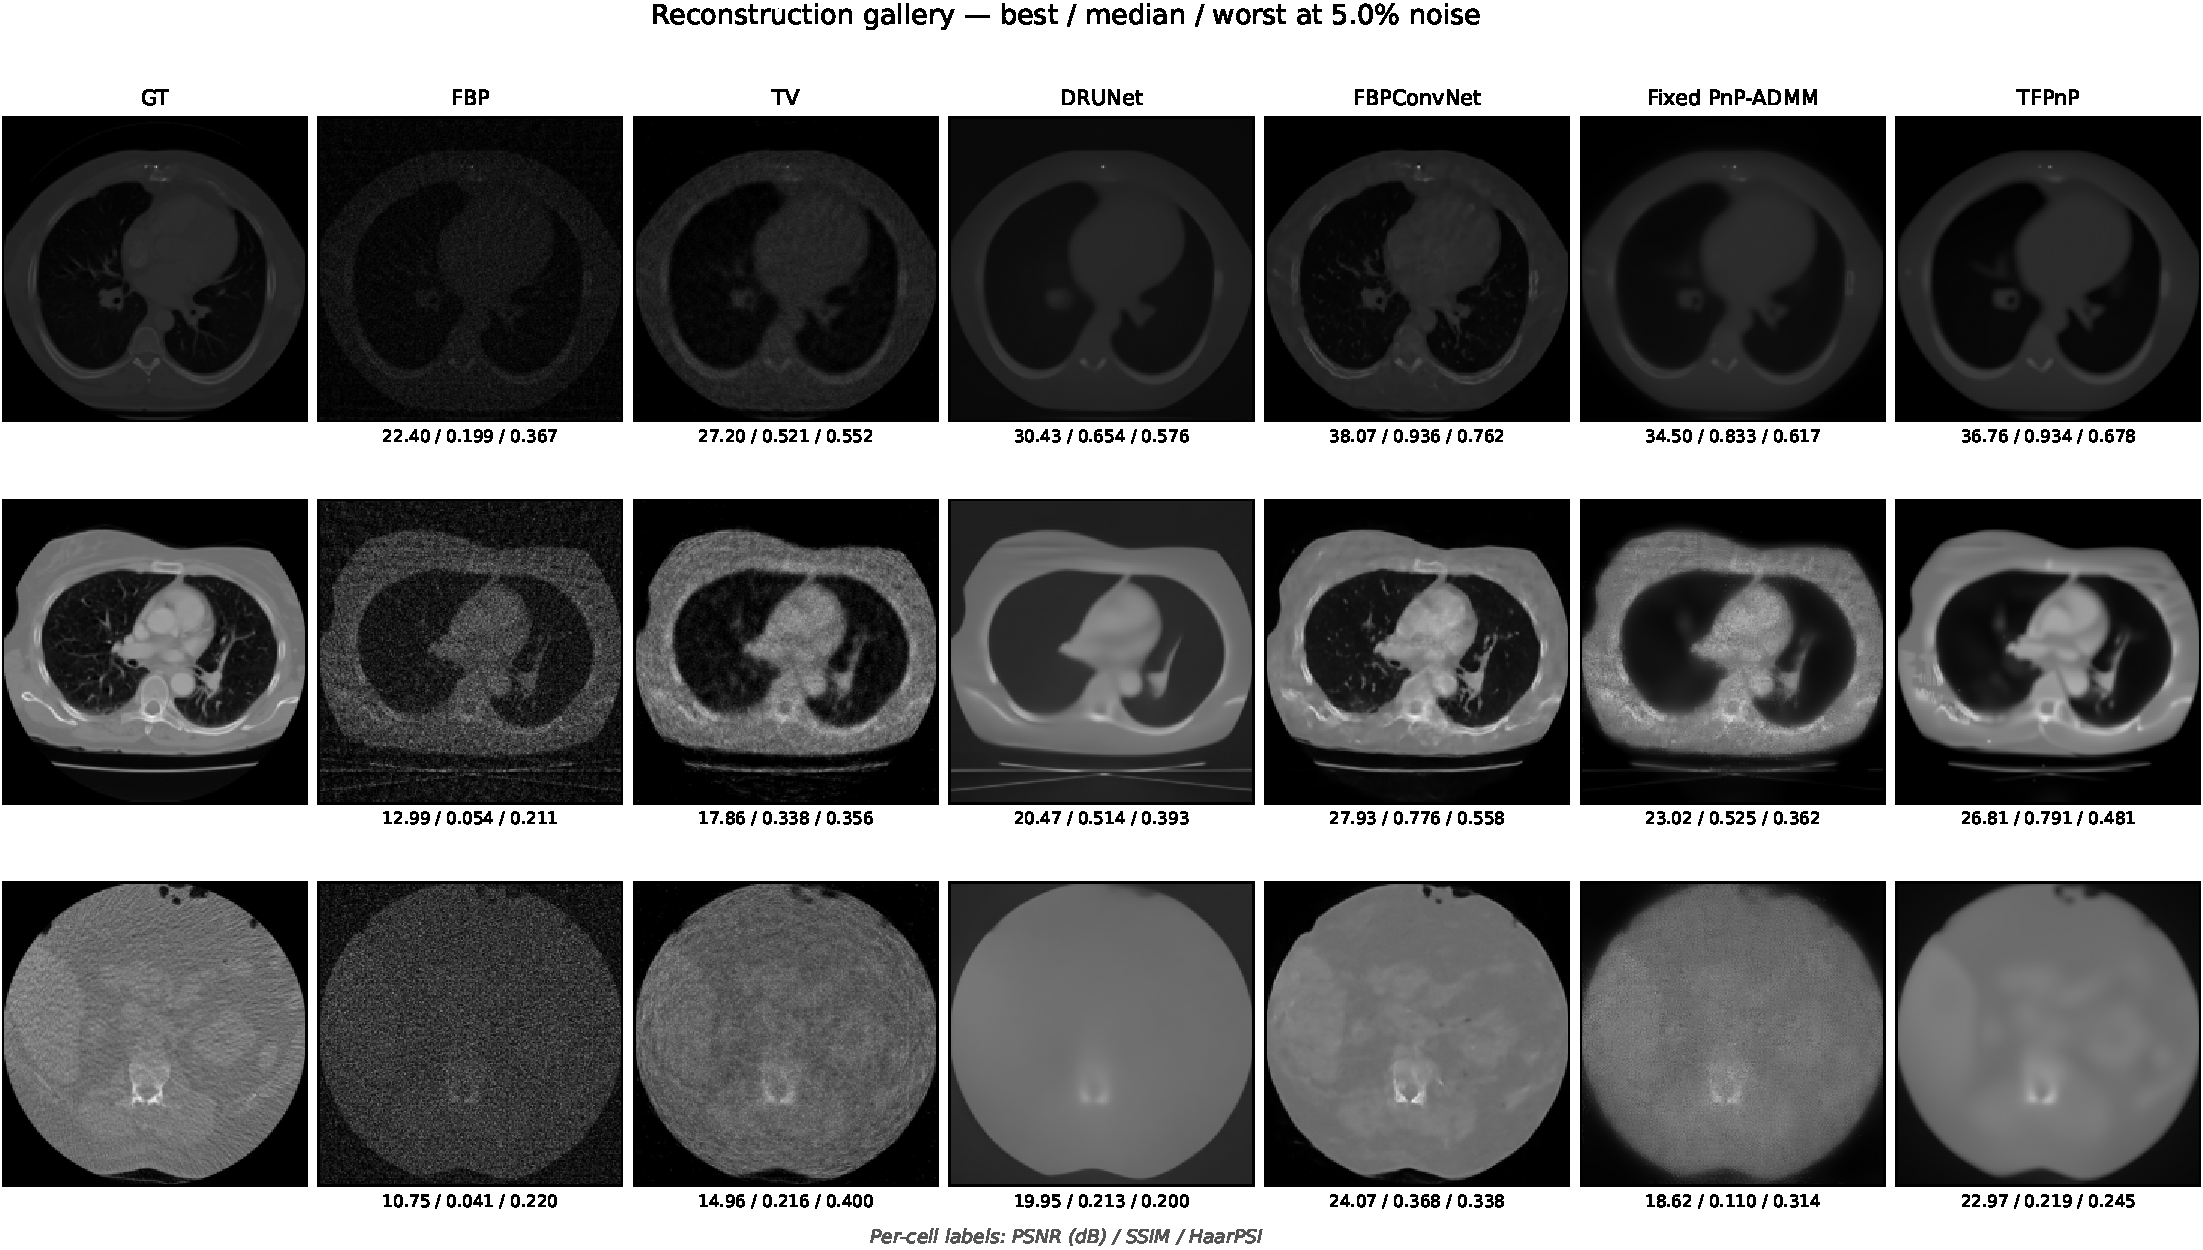
\includegraphics[width=\linewidth]{../figures/run_04_pat_250_e80/gallery.pdf}
    \caption{Reconstruction gallery for \texttt{run\_04} at 5\% noise.
    Rows: best, median, and worst test images by TFPnP PSNR.
    Per-cell labels give PSNR, SSIM, and HaarPSI.}
    \label{fig:reconstruction_gallery}
\end{figure}

% ============================================================
%  Section 4.2 — Cross-noise behaviour
% ============================================================
\section{Cross-noise behaviour}
\label{sec:cross-noise}

TFPnP's practical value depends not only on its performance at the training noise level but also on how well it generalises across the noise range seen at inference. \Cref{fig:metrics_vs_noise} traces mean PSNR, SSIM, and HaarPSI as sinogram noise increases from 5\% to 10\%. TFPnP degrades gracefully, with PSNR dropping only $-1.17$\,dB (from $27.27$ to $26.10$) and SSIM remains effectively flat ($0.691$ to $0.676$). This robustness reflects the strength of the plug-and-play iterative approach, since the policy can adapt the denoising strength
and penalty parameter to different noise levels, rather than producing a single fixed reconstruction.

By contrast, FBPConvNet degrades steeply across the same range ($-3.85$\,dB PSNR, SSIM from $0.726$ to $0.463$), and TFPnP overtakes it on all three metrics at $10\%$ noise. This is partly due to a methodological difference, as our FBPConvNet was trained at a fixed 5\% noise level (\Cref{sec:baselines}) and extrapolates at higher noise. However, the crossover on perceptual metrics at $10\%$ suggests that the iterative structure of TFPnP provides a robustness that training-distribution matches alone would not explain, and is analysed further in~\Cref{sec:why-fbpconvnet}.

% ------------------------------------------------------------
%  Figure 4.2: Metrics vs noise level line plot
% ------------------------------------------------------------
\begin{figure}[H]
    \centering
    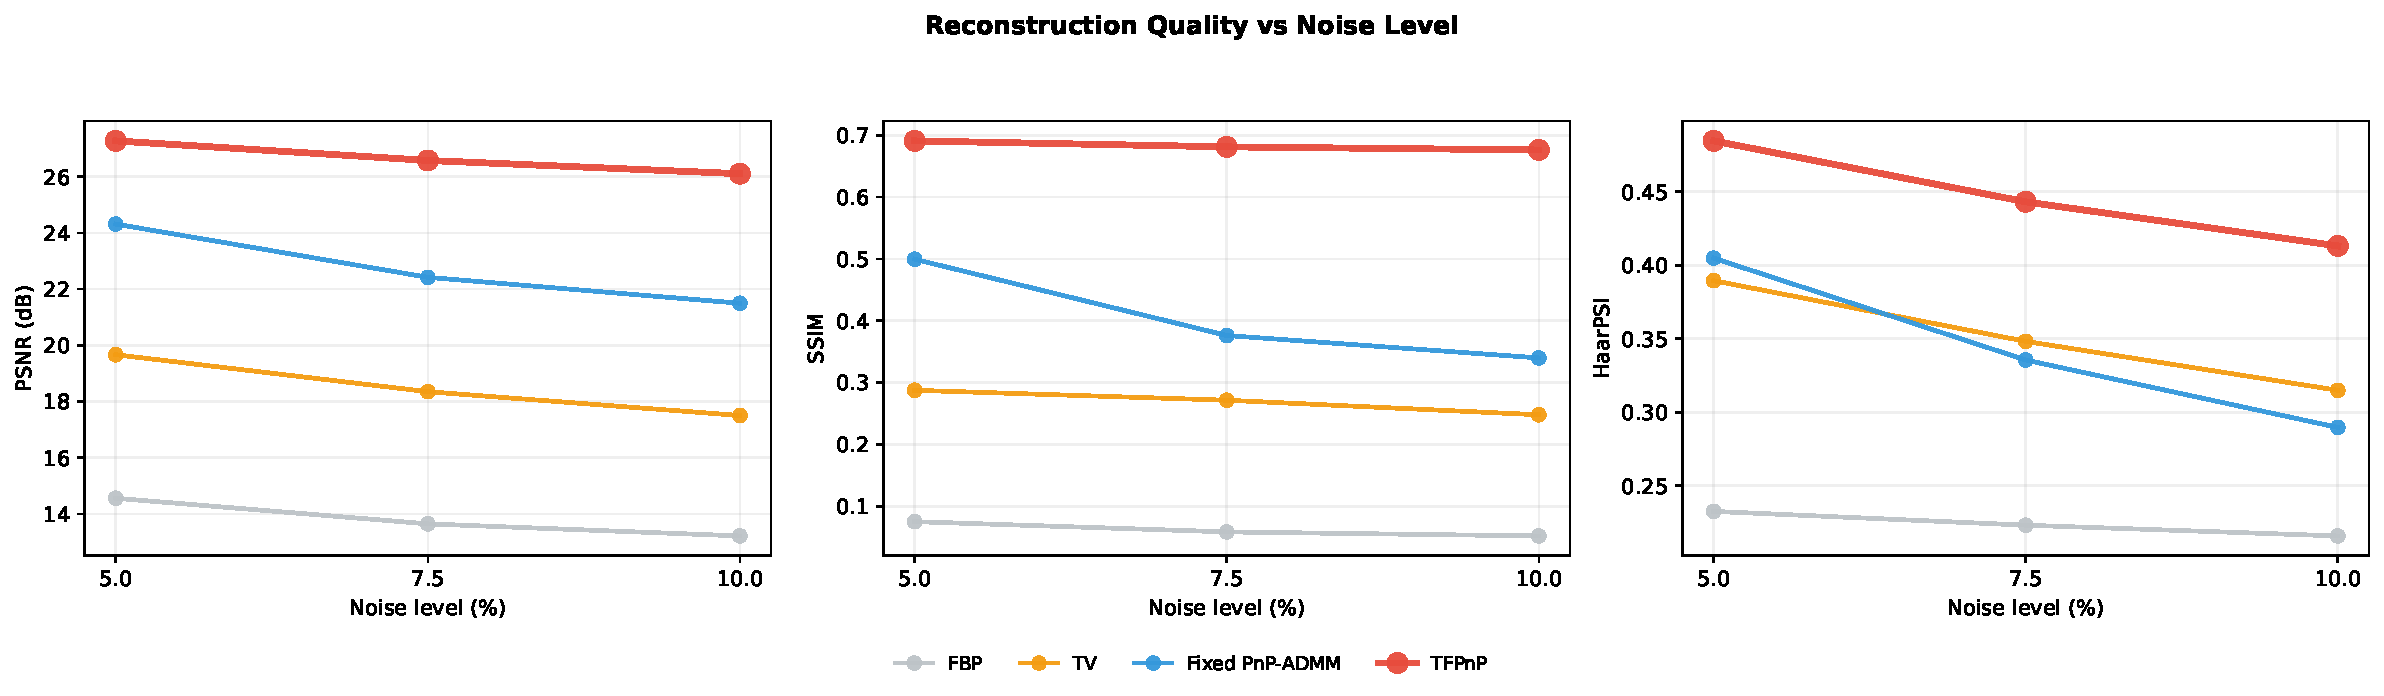
\includegraphics[width=\linewidth]{../figures/run_04_pat_250_e80/metrics_vs_noise.pdf}
    \caption{Mean PSNR, SSIM, and HaarPSI vs sinogram noise level.
    TFPnP overtakes FBPConvNet on all three metrics at 10\% noise.}
    \label{fig:metrics_vs_noise}
\end{figure}

% ============================================================
%  Section 4.3 — Per-image variance
% ============================================================
\section{Per-image variance}
\label{sec:per-image}

Averaging hides per-image variability. \Cref{fig:per_image_psnr} shows TFPnP's three largest wins and losses over the next-best non-TFPnP method at $5\%$ noise, ranked by per-image PSNR delta. TFPnP's wins tend to occur on homogeneous slices with large uniform regions, while losses occur on complex slices with high-frequency detail such as multiple small nodules or intricate anatomy that doesn't contain the lungs. Per-image variability (standard deviations of $\sim 1.5$--$2$\,dB across all methods) means no method dominates uniformly, and reconstructions of comparable quality across methods are common. This is consistent with the general finding that PnP and end-to-end methods have complementary strengths, with neither uniformly outperforming the other.

% ------------------------------------------------------------
%  Figure 4.3: Per-image PSNR bar chart
% ------------------------------------------------------------
\begin{figure}[H]
    \centering
    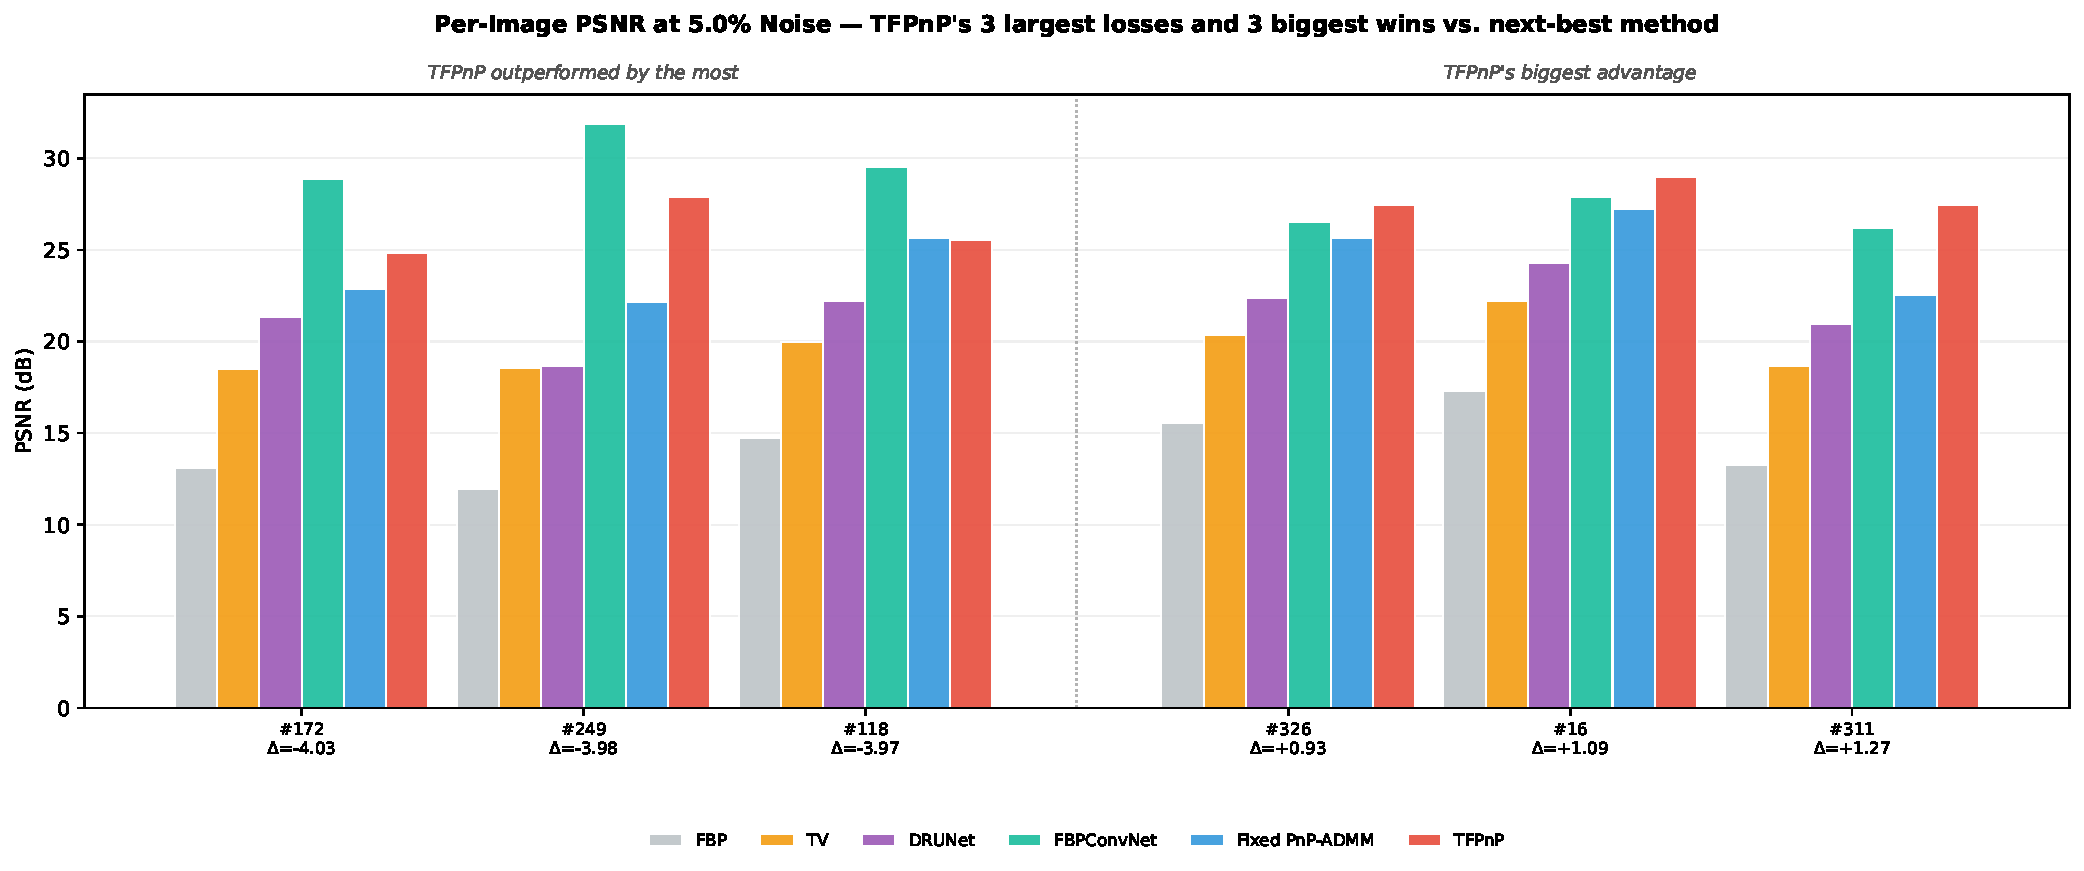
\includegraphics[width=\linewidth]{../figures/run_04_pat_250_e80/per_image_psnr.pdf}
    \caption{Per-image PSNR at 5\% noise. TFPnP's three largest wins
    (left) and losses (right) versus the next-best non-TFPnP method.
    Homogeneous slices favour TFPnP, complex ones favour FBPConvNet.}
    \label{fig:per_image_psnr}
\end{figure}

% ============================================================
%  Section 4.4 — Hyperparameter calibration sweeps
% ============================================================
\section{Hyperparameter calibration sweeps}
\label{sec:calibration}

The Fixed PnP-ADMM baseline uses hand-calibrated $\sigma = 1.5$ and $\mu = 20$ values for the natural-image DRUNet, identified through sensitivity sweeps during notebook development. When the denoiser is swapped for the CT-trained DRUNet developed in~\Cref{sec:ct-drunet}, this calibration is no longer valid, and~\Cref{fig:sigma_sweep_natural} and~\Cref{fig:sigma_sweep_ct} present calibration sweeps for both denoisers. The CT-trained DRUNet peaks at $\sigma = 8.0$ in the wrapper's units; the interpretation of this apparent shift is revisited in~\Cref{sec:corrections}. The corresponding $\mu$ sweep at $\sigma = 8$ (see~\Cref{fig:mu_sweep_ct}) reveals a peak at $\mu = 10$, half the natural-DRUNet value.

Two limitations of these sweeps are worth noting. First, they were performed on a single representative slice at 5\% noise, and a broader sweep across the validation set was intended but could not be completed within the available compute budget. Second, the sweep grids used $\sigma \in [1, 25]$ and $\mu \in [5, 50]$, but a finer grid around the peak could refine the calibration further.

% ------------------------------------------------------------
%  Figure 4.4a: σ sensitivity sweep — natural DRUNet
% ------------------------------------------------------------
\begin{figure}[H]
    \centering
    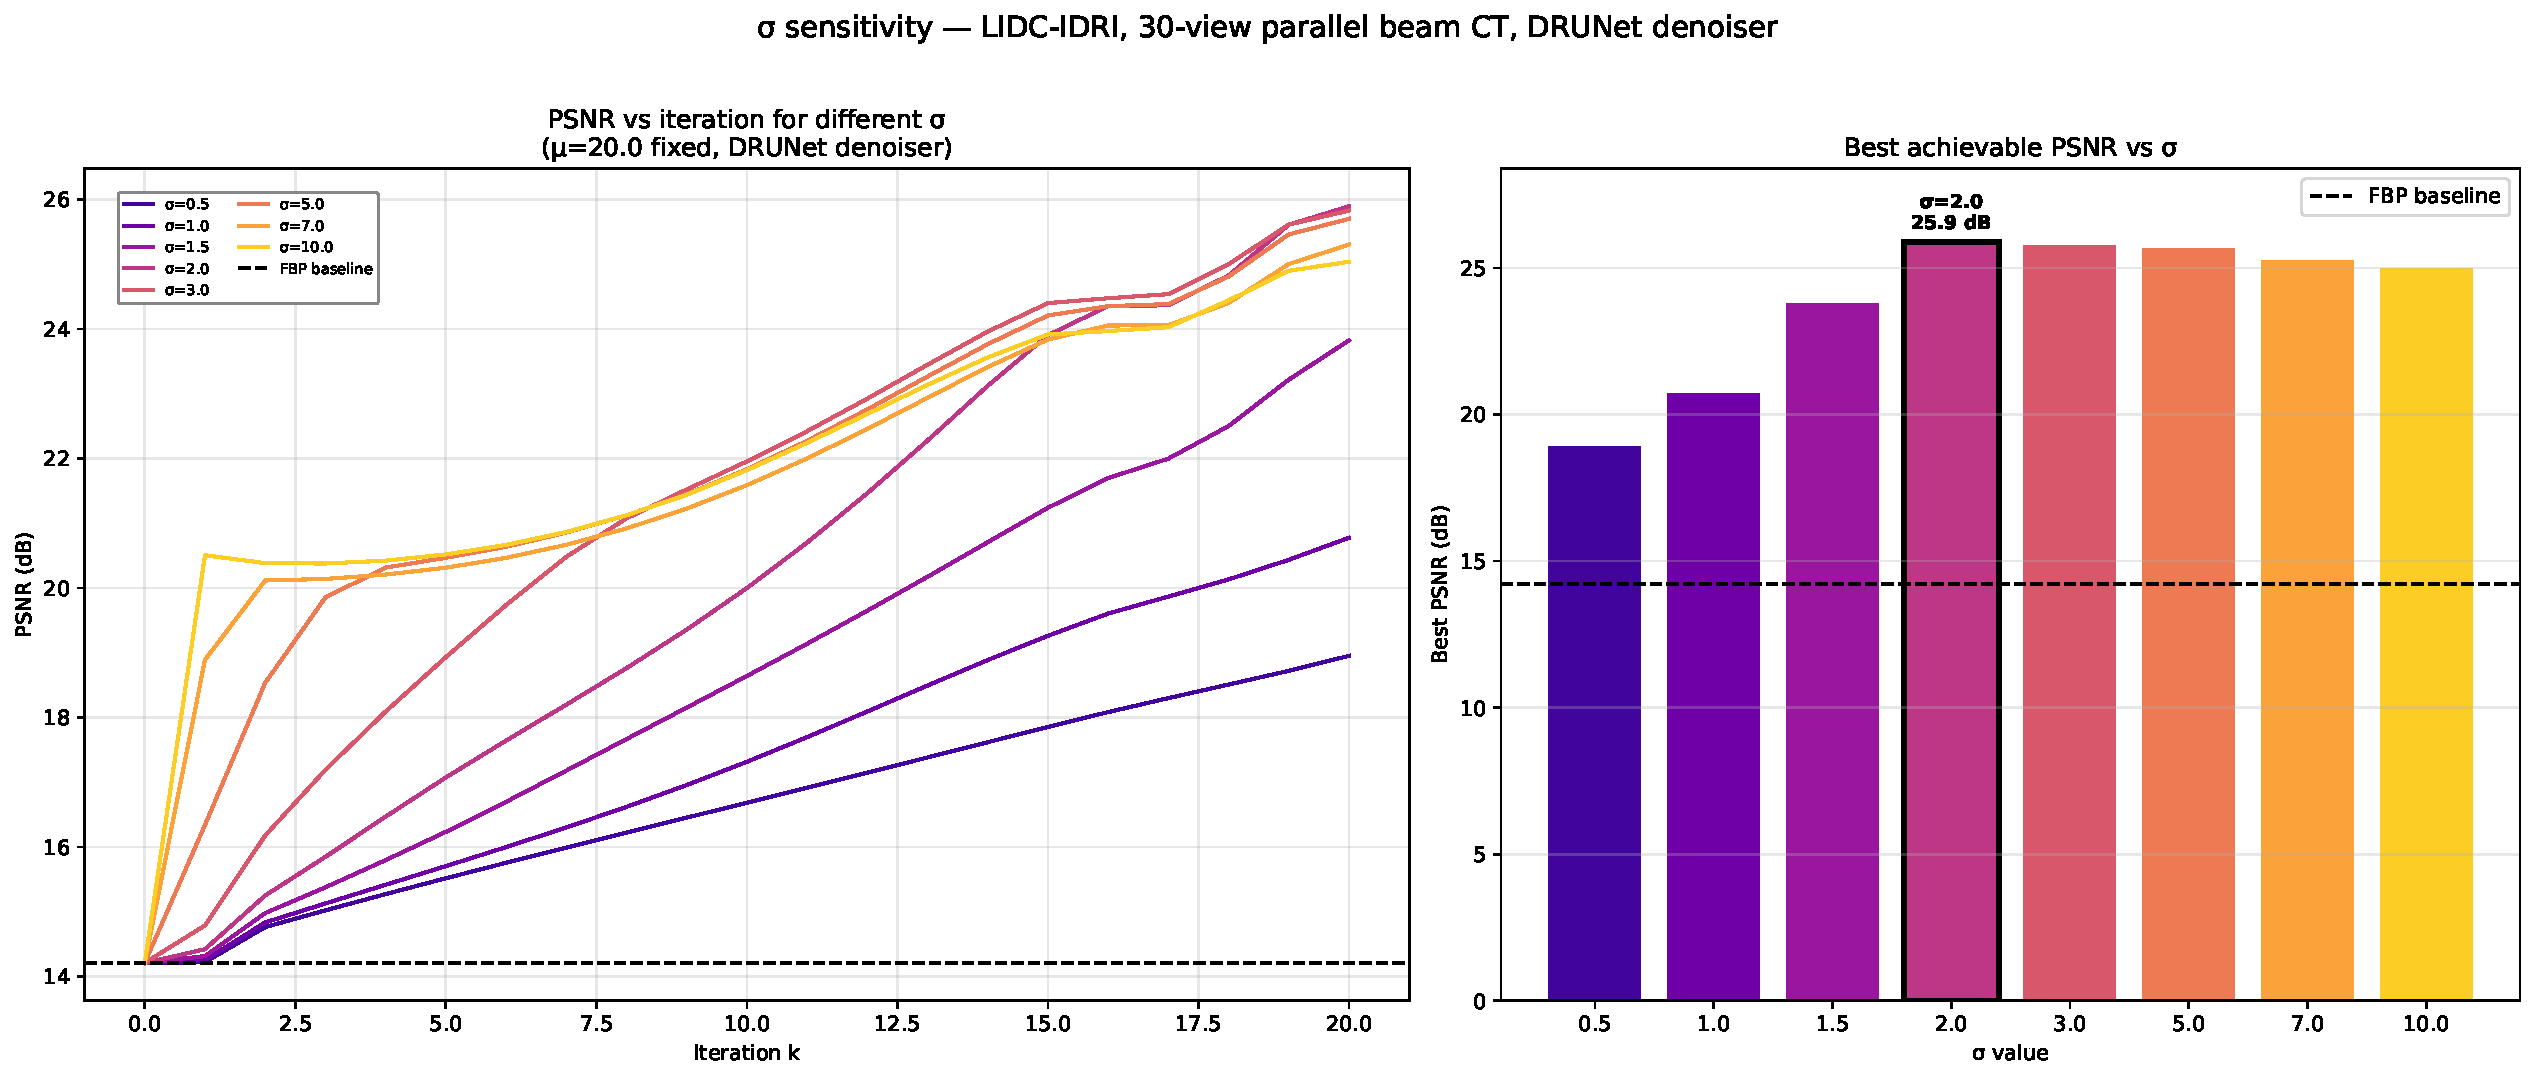
\includegraphics[width=\linewidth]{../figures/05/07_sigma_sensitivity.pdf}
    \caption{$\sigma$ sensitivity for natural-image DRUNet within Fixed
    PnP-ADMM at 5\% noise. Peak at $\sigma = 1.5$.}
    \label{fig:sigma_sweep_natural}
\end{figure}

% ------------------------------------------------------------
%  Figure 4.4b: σ sensitivity sweep — CT DRUNet
% ------------------------------------------------------------
\begin{figure}[H]
    \centering
    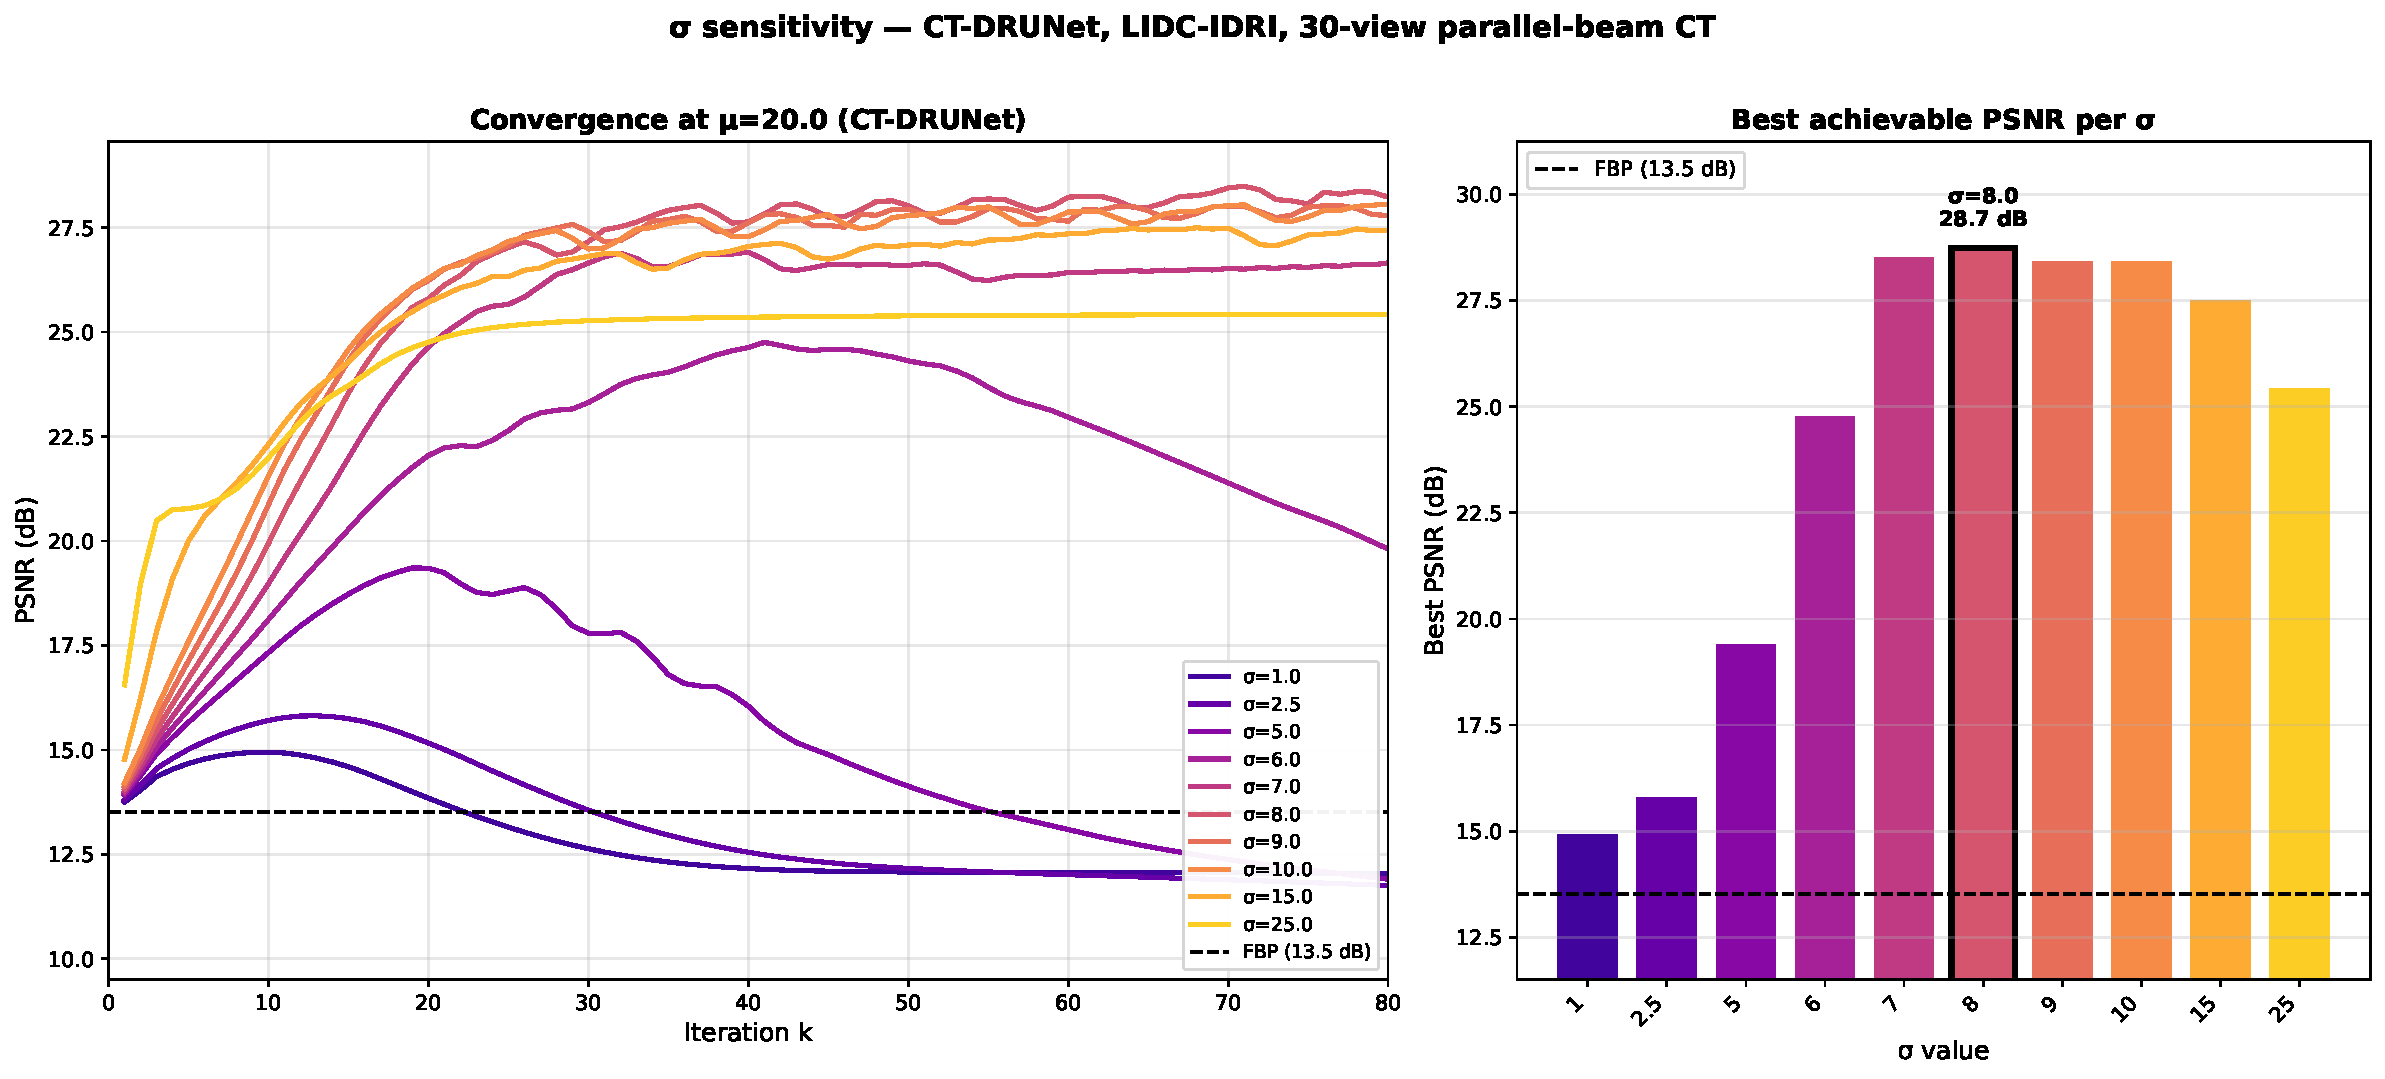
\includegraphics[width=\linewidth]{../figures/12/06_sigma_sensitivity_ctdrunet.pdf}
    \caption{$\sigma$ sensitivity for CT-trained DRUNet within Fixed PnP-ADMM
    at 5\% noise. Peak at $\sigma = 8.0$.}
    \label{fig:sigma_sweep_ct}
\end{figure}

% ------------------------------------------------------------
%  Figure 4.4c: µ sensitivity sweep — CT DRUNet at σ=8
% ------------------------------------------------------------
\begin{figure}[H]
    \centering
    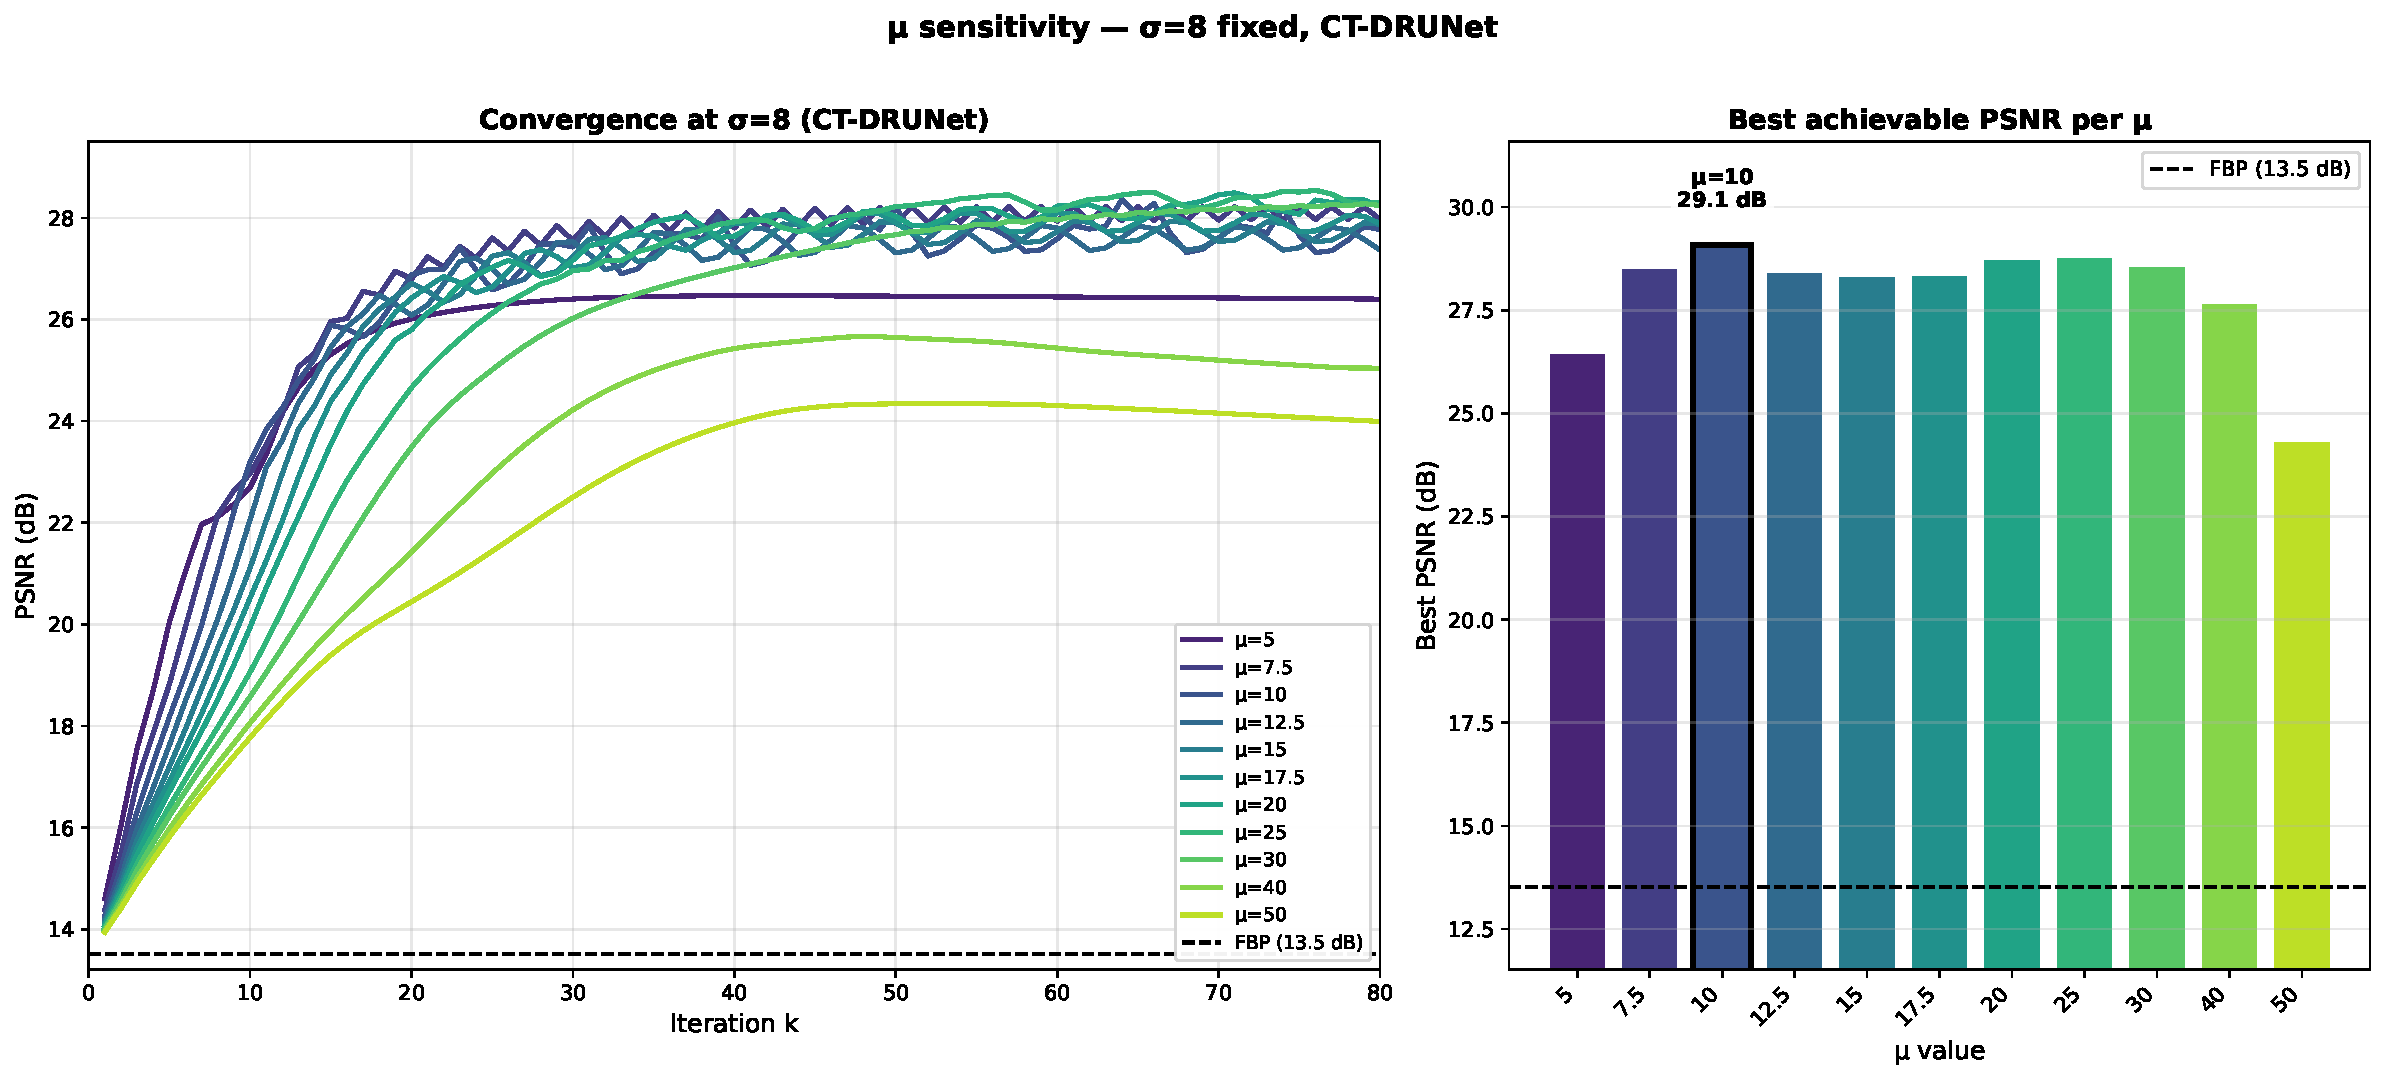
\includegraphics[width=\linewidth]{../figures/12/07_mu_sensitivity_ctdrunet.pdf}
    \caption{$\mu$ sensitivity for CT-trained DRUNet at $\sigma = 8$. Peak
    at $\mu = 10$.}
    \label{fig:mu_sweep_ct}
\end{figure}

% ============================================================
%  Section 4.5 — In-domain denoiser experiment
% ============================================================
\section{In-domain denoiser experiment}
\label{sec:in-domain}

With the CT-trained DRUNet calibrated to its own operating point ($\sigma = 8$, $\mu = 10$), a paired comparison of Fixed PnP-ADMM using each denoiser at its respective optimum was performed on the full 389-image test set (\Cref{tab:fixed_pnp_ct_vs_natural}). The CT-DRUNet outperforms the natural-image DRUNet at every noise level, and the advantage grows with noise, from $+0.71$\,dB at 5\% to $+1.98$\,dB at 10\%. SSIM improvements follow the same trend, from $+0.037$ to $+0.090$.

The advantage grows with noise; its interpretation is discussed in~\Cref{sec:in-domain-gap}. \Cref{fig:fixed_pnp_optimum_comparison} shows a visual comparison at all three noise levels.

This comparison uses Fixed PnP-ADMM rather than TFPnP with the learned policy, as retraining the policy against the CT denoiser (\Cref{sec:run11}) encountered training instability that could not be resolved before a CSD3 cluster outage.

% ------------------------------------------------------------
%  Table 4.3: Fixed PnP-ADMM — natural vs CT-DRUNet at each optimum
% ------------------------------------------------------------
\begin{table}[H]
    \centering
    \footnotesize
    \caption{Fixed PnP-ADMM at each denoiser's calibrated optimum.}
    \label{tab:fixed_pnp_ct_vs_natural}
    \begin{tabular}{lcc cc cc cc}
        \toprule
        & \multicolumn{2}{c}{\textbf{5\% noise}}
        & \multicolumn{2}{c}{\textbf{7.5\% noise}}
        & \multicolumn{2}{c}{\textbf{10\% noise}}
        & \multicolumn{2}{c}{\textbf{Advantage}} \\
        \cmidrule(lr){2-3} \cmidrule(lr){4-5} \cmidrule(lr){6-7} \cmidrule(lr){8-9}
        Denoiser        & PSNR  & SSIM  & PSNR  & SSIM  & PSNR  & SSIM  & PSNR  & SSIM  \\
        \midrule
        Natural DRUNet ($\sigma{=}1.5$) & 28.06 & 0.752 & 26.52 & 0.695 & 25.41 & 0.652 & -- & -- \\
        CT DRUNet ($\sigma{=}8$)       & \textbf{28.77} & \textbf{0.789} & \textbf{27.91} & \textbf{0.768} & \textbf{27.39} & \textbf{0.742} & $+0.71$ to $+1.98$ & $+0.037$ to $+0.090$ \\
        \bottomrule
    \end{tabular}
\end{table}

% ------------------------------------------------------------
%  Figure 4.6: Fixed PnP-ADMM at optimum comparison
% ------------------------------------------------------------
\begin{figure}[H]
    \centering
    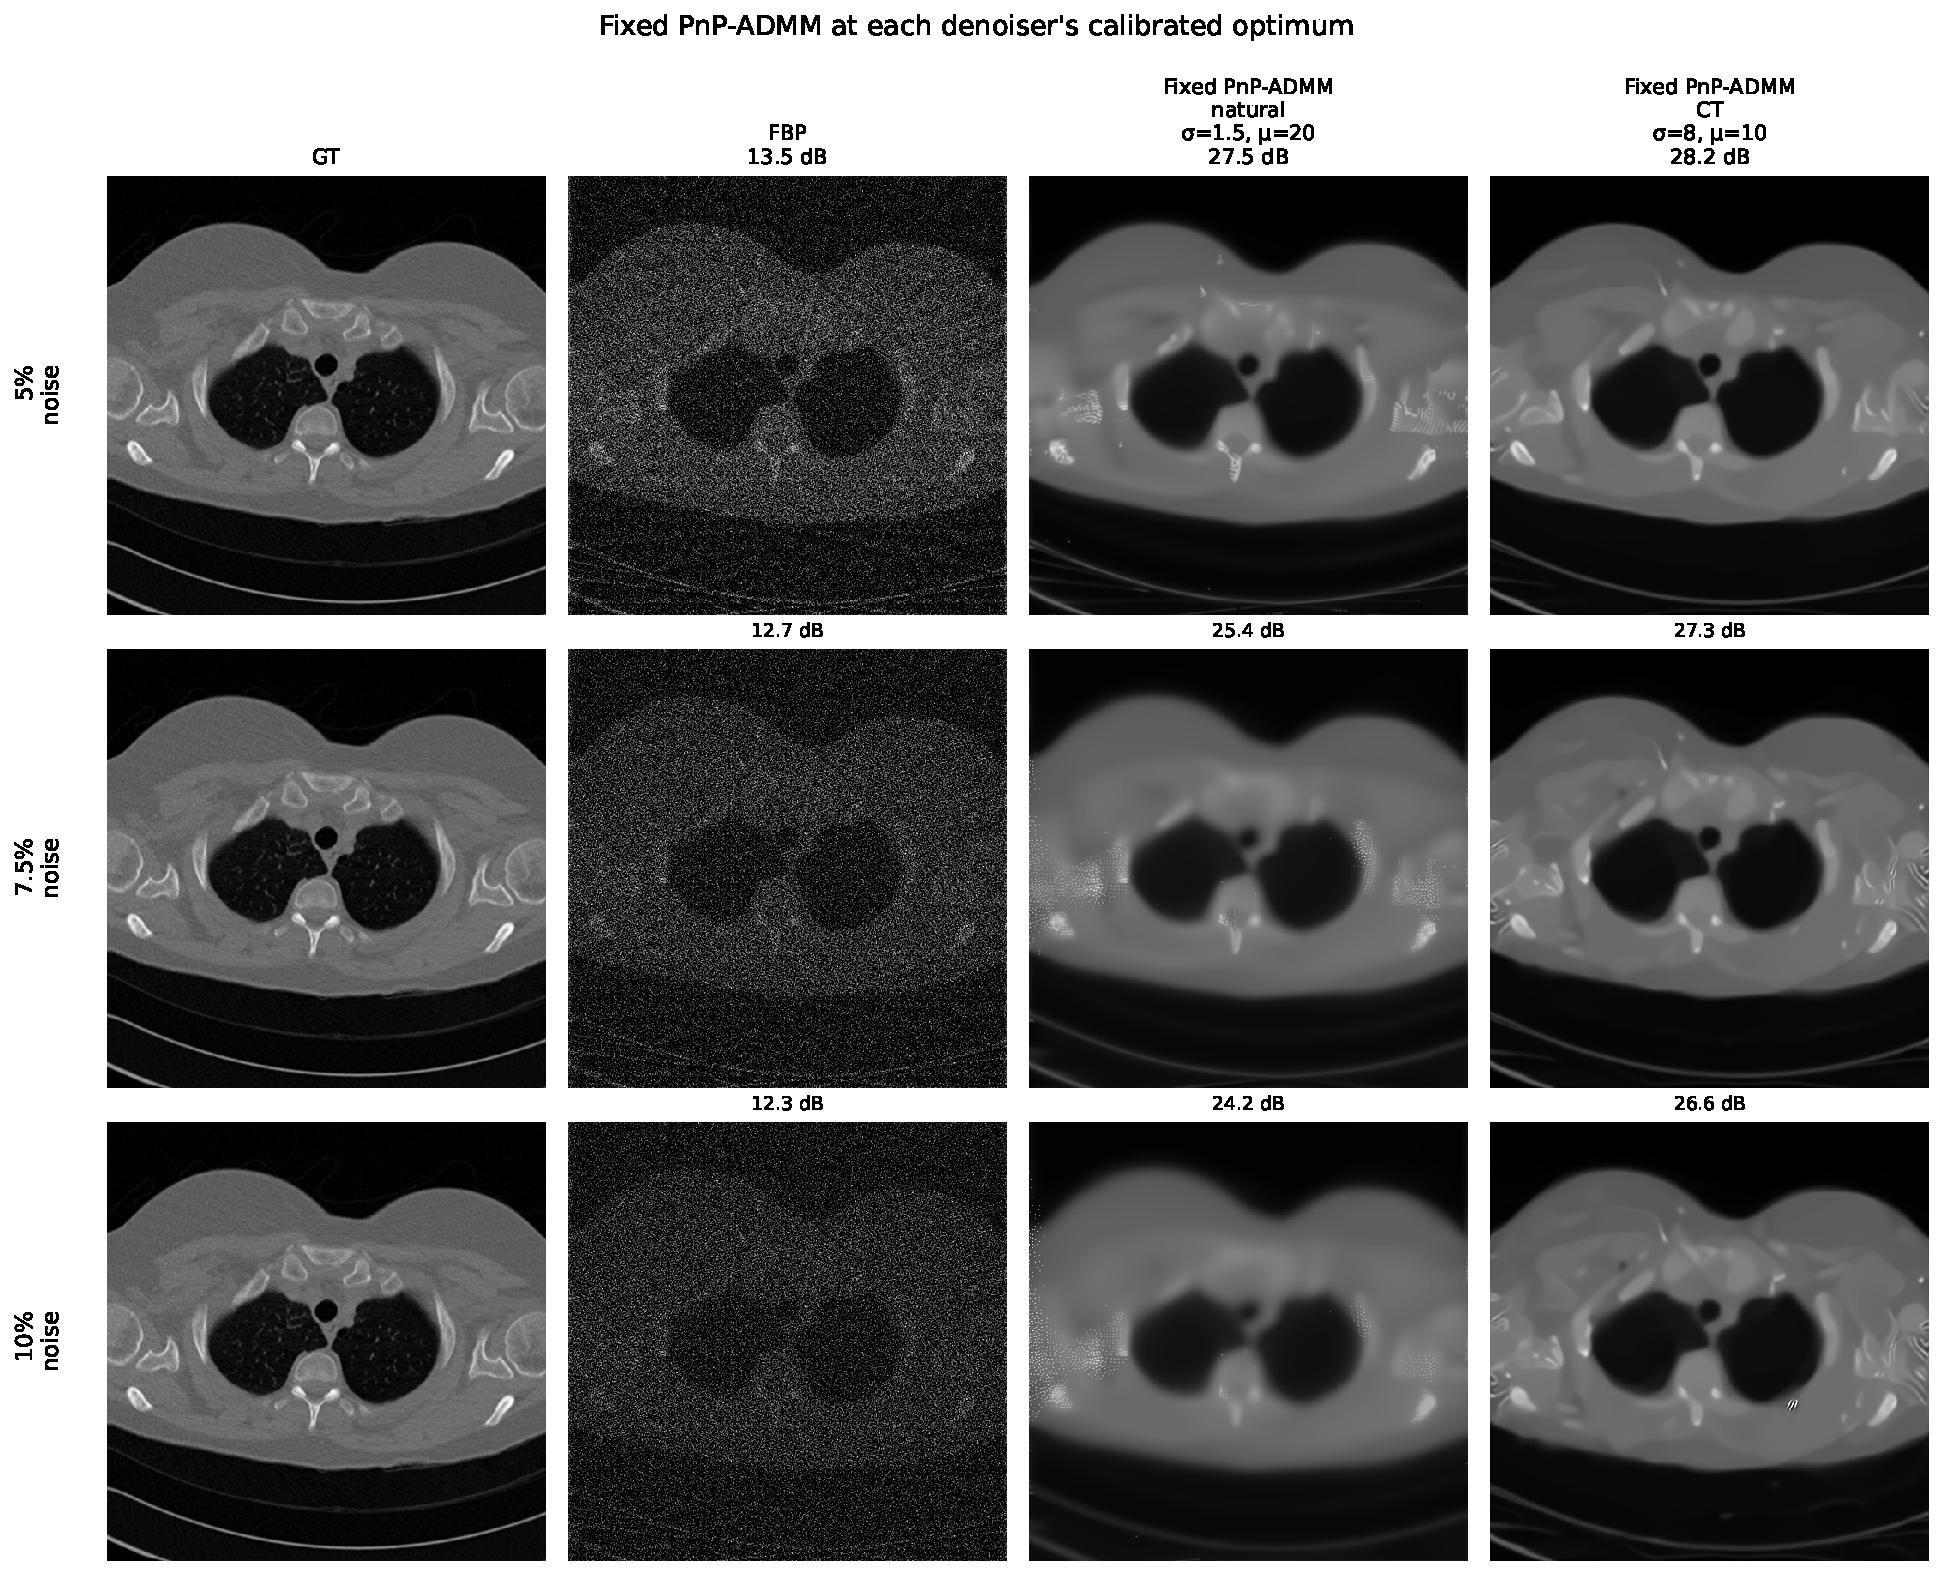
\includegraphics[width=\linewidth]{../figures/12/08_fixed_pnp_optimum_comparison.pdf}
    \caption{Fixed PnP-ADMM with denoisers at their calibrated optimum, at 5\%, 7.5\%, and 10\% noise.}
    \label{fig:fixed_pnp_optimum_comparison}
\end{figure}

% ============================================================
%  Section 4.6 — TFPnP policy retrain with CT-DRUNet
% ============================================================
\section{TFPnP policy retrain with CT-DRUNet}
\label{sec:run11}

The natural next step is retraining the TFPnP policy against the CT-DRUNet, with a widened $\sigma$ action range $[1, 15]$ to cover the new optimum and a narrowed $\mu$ range $[5, 50]$ chosen to keep the ADMM balance stable at the higher $\sigma$ values. This run (\texttt{run\_11}) underperformed \texttt{run\_04}, reaching only $26.51$\,dB at 5\% noise, well below \texttt{run\_04}'s $27.27$\,dB and below even the Fixed PnP-ADMM baseline with CT-DRUNet at $28.77$\,dB (\Cref{sec:in-domain}).

\Cref{fig:run11_training_curves} shows the diagnostic training curves. Around policy update step 15{,}000, the critic loss explodes to $10^{19}$-scale magnitudes, the policy's mean $\sigma$ output drifts from $\sim 14$ to $\sim 9$, and both training and validation PSNR collapse from their earlier trajectory. The best checkpoint is saved from epoch 1, indicating no improvements were made. Since both the $\sigma$ and $\mu$ ranges were changed simultaneously, the failure cannot be attributed to either alone, but the drift in the policy's mean $\sigma$ output suggests the widened action space is the more likely cause. A third factor cannot be excluded. Our value network omits the weight normalisation and TReLU that Table~1 of~\citet{Wei2022TFPnP} specifies for the critic (\Cref{sec:tfpnp-policy}), and both are adopted in their source papers for their stabilising effect on training. Whether the divergence follows from the widened action range, from this architectural omission, or from both, could not be separated at the time. A post-hoc diagnosis identifying a further, more fundamental cause is given in~\Cref{sec:corrections}.

% ------------------------------------------------------------
%  Figure 4.5: run_11 training curves
% ------------------------------------------------------------
\begin{figure}[H]
    \centering
    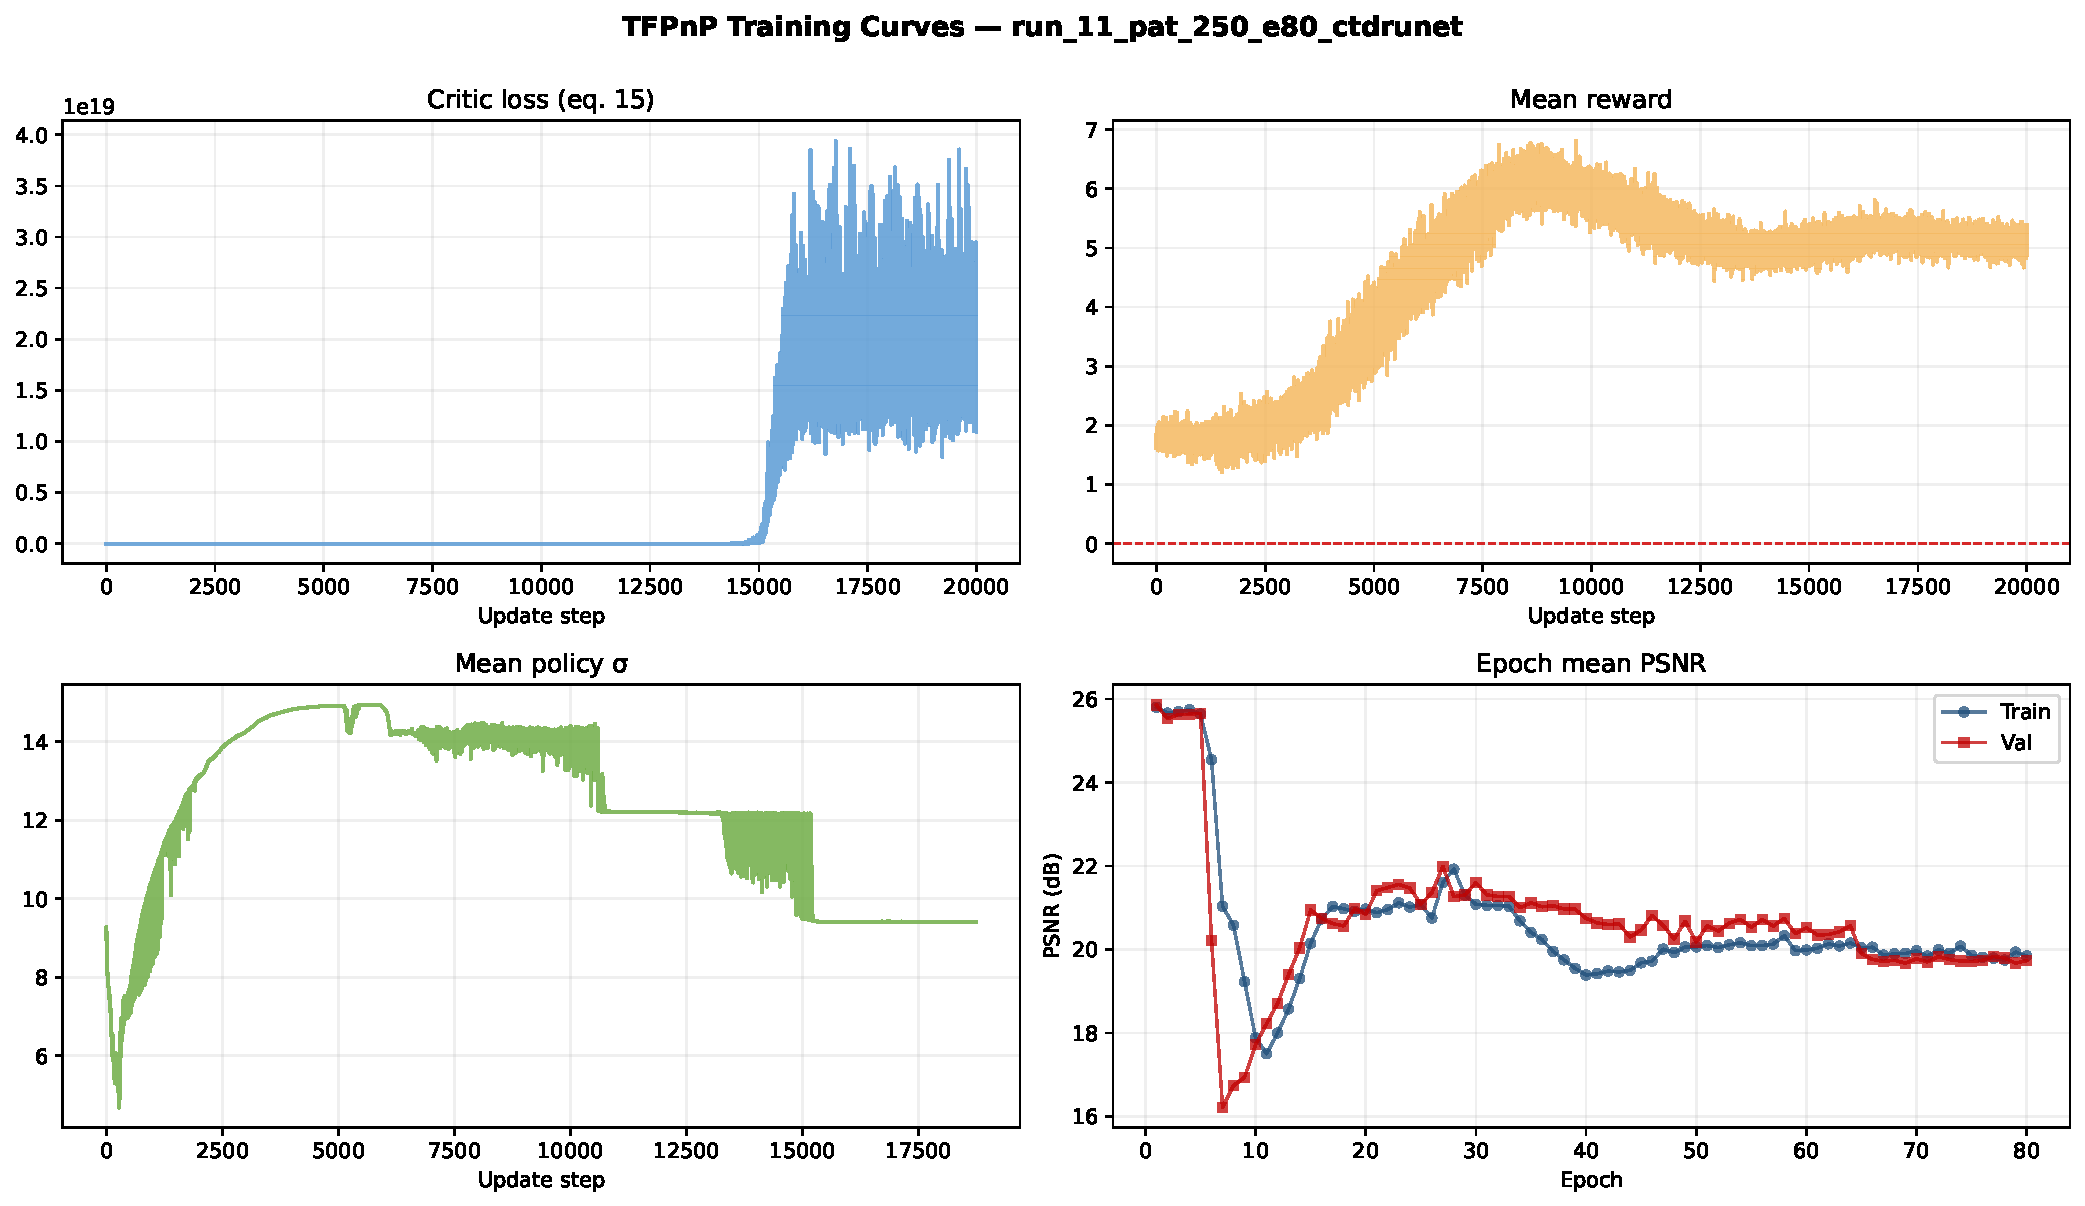
\includegraphics[width=\linewidth]{../figures/run_11_pat_250_e80_ctdrunet/training_curves.pdf}
    \caption{Training curves for \texttt{run\_11}.}
    \label{fig:run11_training_curves}
\end{figure}

% ============================================================
%  Section 4.7 — Reward shaping ablations
% ============================================================
\section{Reward shaping ablations}
\label{sec:reward-shaping}

Four variant runs were carried out to test whether alternative reward signals could improve metric-specific performance, motivated by the finding of~\citet{breger2025study} that PSNR correlates poorly with perceived image quality in medical imaging, raising the question of whether an RL policy rewarded on different metrics would produce better reconstructions than one trained on PSNR alone. The study is an extension undertaken in addition to the reproduction, rather than a component of~\citet{Wei2022TFPnP}'s original methodology, and results are summarised in~\Cref{tab:reward_shaping}.

The reward coefficients compensate for the difference in numeric scale between metrics. A typical per-step $\Delta\text{PSNR}$ is on the order of $0.1$--$1.0$, whereas $\Delta\text{SSIM}$ and $\Delta\text{HaarPSI}$ are on the order of $0.001$--$0.01$, so without scaling, the they would be roughly $100\times$ smaller than the PSNR term and contribute negligibly to the policy gradient. The mixed rewards (\texttt{run\_07}, \texttt{run\_08}) therefore use $\alpha = 5$ to bring the perceptual term to a comparable order of magnitude as $\Delta\text{PSNR}$, and the pure-replacement rewards (\texttt{run\_09}, \texttt{run\_10}) use $\alpha = 50$ so the overall reward magnitude remains comparable to \texttt{run\_04}'s pure-PSNR reward.

The SSIM-only reward (\texttt{run\_09}) achieves the highest PSNR and HaarPSI among all runs, and the mixed PSNR/SSIM reward (\texttt{run\_07}) wins on SSIM specifically. In contrast, both HaarPSI-based rewards (\texttt{run\_08} PSNR/HaarPSI, \texttt{run\_10} HaarPSI only) underperform across all metrics. Given only a single training seed per configuration, some of this variation likely reflects RL training stochasticity rather than the differences between reward functions, so the PSNR reward chosen for \texttt{run\_04} remains a defensible default for direct comparison to the paper.

% ------------------------------------------------------------
%  Table 4.4: Reward-shaping ablation summary (runs 07-10)
% ------------------------------------------------------------
\begin{table}[H]
    \centering
    \footnotesize
    \caption{Reward-shaping ablation at 5\% noise. Best values in \textbf{bold}.}
    \label{tab:reward_shaping}
    \begin{tabular}{llccc}
        \toprule
        Run & Reward function & PSNR & SSIM & HaarPSI \\
        \midrule
        \texttt{run\_04} & PSNR (main)     & 27.27          & 0.691          & 0.485          \\
        \texttt{run\_07} & PSNR + SSIM     & 27.18          & \textbf{0.707} & 0.481          \\
        \texttt{run\_08} & PSNR + HaarPSI  & 26.47          & 0.640          & 0.437          \\
        \texttt{run\_09} & SSIM only       & \textbf{27.32} & 0.695          & \textbf{0.489} \\
        \texttt{run\_10} & HaarPSI only    & 26.76          & 0.658          & 0.460          \\
        \bottomrule
    \end{tabular}
\end{table}


% ==============================================================================
% Chapter 5: Discussion
% ==============================================================================
% ============================================================
%  Chapter 5: Discussion
% ============================================================

\chapter{Discussion}
\label{chap:discussion}

% ============================================================
%  Section 5.1
% ============================================================
\section{Contextualising the TFPnP–FBPConvNet comparison}
\label{sec:why-fbpconvnet}

The reproduction confirms~\citet{Wei2022TFPnP}'s central claims. The learned policy improves on hand-calibrated hyperparameters by $+2.96$\,dB at 5\% noise (\Cref{sec:headline}), and TFPnP degrades gracefully across the noise range (\Cref{sec:cross-noise}). The one direct disagreement with the paper is the FBPConvNet–TFPnP ranking at 5\% noise, which reverss, but can be explained by two factors.

The first is an in-domain training asymmetry. In~\citet{Wei2022TFPnP}, TFPnP's denoiser is trained on BSD400 and its policy on PASCAL VOC, both natural-image datasets. FBPconv's training data is not stated explicitly, but the paper's relativedly flat FBPconv PSNRs across noise levels ($23.00, 22.94, 22.86$\,dB) are consistent with out-of-domain training. In this reproduction, FBPConvNet is trained end-to-end on LIDC, while TFPnP's policy is also LIDC-trained but the denoiser remains the natural-image DRUNet (\Cref{tab:implementation-differences}). FBPConvNet is fully in-domain, yet TFPnP is only partially so, and at low noise the fully in-domain method extracts fine anatomical detail from the FBP reconstruction more effectively than the natural-image denoiser can.

The second is architectural. TFPnP overtakes FBPConvNet at 10\% noise on all three metrics (\Cref{fig:metrics_vs_noise}), with a PSNR drop across the range ($-1.17$\,dB) roughly a third of FBPConvNet's ($-3.85$\,dB). Part of this reflects a training-distribution effect, as FBPConvNet was trained at fixed 5\% noise while TFPnP saw the mixed regime, but the crossover on SSIM and HaarPSI is unlikely to be explained by that alone. Repeated denoising passes appear to remove sinogram noise progressively in a way a single forward pass cannot. The paper's out-of-domain comparison obscured both effects, flattering TFPnP relative to FBPconv on the averaged ranking.

% ============================================================
%  Section 5.2
% ============================================================
\section{Does an in-domain denoiser close the gap?}
\label{sec:in-domain-gap}

If FBPConvNet's advantage at low noise comes from its in-domain training, a natural extension is to give TFPnP the same advantage by training the denoiser on CT rather than natural images. The CT-DRUNet extension experiment (\Cref{sec:ct-drunet}) yields two findings and one negative result.

The first finding is that in the Fixed PnP-ADMM setting, the CT-trained DRUNet outperforms the natural-image DRUNet at every noise level, with the advantage growing with noise (\Cref{tab:fixed_pnp_ct_vs_natural}). This result stands independently of what happens with the full TFPnP pipeline.

The second is that the CT-DRUNet operates at a fundamentally different $\sigma$ scale than the natural-image DRUNet. The natural DRUNet peaks at $\sigma = 1.5$ (\Cref{fig:sigma_sweep_natural}), the CT-DRUNet at $\sigma = 8.0$ (\Cref{fig:sigma_sweep_ct}). Domain-specific training therefore does not just refine the denoiser's ability to reject noise, but shifts the operating point at which the denoiser is most useful, with direct consequences for how policy $\sigma$ ranges must be configured when swapping denoisers within TFPnP.

The negative result is that retraining the TFPnP policy against the CT-DRUNet (\texttt{run\_11}) with a widened $\sigma$ action range failed. The critic loss diverged and the policy $\sigma$ output collapsed shortly afterwards. The obvious explanation is the action range itself, as widening $\sigma$ from $[1, 5]$ to $[1, 15]$ enlarges the space of reachable ADMM states, and therefore the range of values the critic must learn to estimate. A second explanation is our own value network, as Table~1 of~\citet{Wei2022TFPnP} specifies that the critic uses the policy's feature extractor with batch normalisation replaced by weight normalisation and ReLU replaced by TReLU. Our critic removes batch normalisation, as the paper does, but puts nothing in its place, using unnormalised convolutions and standard ReLU activations (\Cref{sec:tfpnp-policy}). Weight normalisation is introduced specifically to stabilise training, but our critic has neither and diverges.

Taken together, these results suggest that the in-domain denoiser advantage is real and reproducible in the simpler Fixed PnP-ADMM setting, but that we were unable to translate it into the RL-based TFPnP pipeline. Whether that reflects a sensitivity of TFPnP's RL formulation to action-range choices, or our own substitution of the value network, remains open.
% ============================================================
%  Section 5.3 — On the choice of evaluation metrics
% ============================================================
\section{On the choice of evaluation metrics}
\label{sec:metrics-discussion}

PSNR is the primary metric throughout this report, and was chosen for direct comparison to~\citet{Wei2022TFPnP}. However, PSNR captures only pixel-wise mean squared error, which does not always correlate with the visual quality in medical imaging. PSNR weights every pixel equally and is insensitive to the structure of errors, so a slightly blurred reconstruction that smooths away texture can score identically to one that preserves texture but adds a small amount of noise, although a radiologist would rate the two very differently. SSIM partially addresses the second issue by comparing local luminance, contrast, and structural patterns rather than only pixel intensities. HaarPSI extends this further through a Haar wavelet decomposition, and has been shown to correlate more strongly with radiological assessment than either PSNR or SSIM~\citep{breger2025study}. 

% ============================================================
%  Section 5.4 — On direct comparison with the paper
% ============================================================
\section{On direct comparison with~\citet{Wei2022TFPnP}}
\label{sec:direct-comparison}

The absolute PSNR values reported in this project cannot be directly compared with those in~\citet{Wei2022TFPnP}, due to the differences detailed below.

First, the PSNR data-range convention differs, with this report following LION's per-image \texttt{data\_range} $= x_{\text{gt}}.\text{max}()$ in native $\mu$ units, whereas the paper does not state its convention but most likely uses \texttt{data\_range} $= 1.0$ on $[0, 1]$-normalised images. This alone accounts for a $\sim 5$\,dB shift in reported PSNR for the same mean squared error (\Cref{sec:geometry-noise}), affecting direct comparisons but not within-experiment rankings.

Second, the paper reports on 50 randomly selected lung slices from the COVID-19 CT lung and infection segmentation dataset, and this project reports on the full 389-image LIDC-IDRI test set. The two datasets have different image statistics, noise characteristics, and anatomy distributions, so absolute PSNR is not directly comparable even at identical noise levels.

Third, the sinogram noise convention differs, as while both the paper and this reproduction follow a percentage-of-signal-standard-deviation convention, the paper's scaling is not documented in detail, so replication is inexact (\Cref{sec:geometry-noise}), but LION's own more physical Poisson-Gaussian noise model was not used to mitigate this issue as much as possible.

Fourth, several implementation choices differ, consolidated in~\Cref{tab:implementation-differences}. The denoiser is trained with MSE loss (\texttt{train\_drunet\_ct.py}) rather than the $L_1$ loss used by~\citet{Wei2022TFPnP} and~\citet{zhang2021plug}, chosen because PSNR is monotone in MSE and so aligns the denoiser with the RL reward $\Delta\text{PSNR}$, at the cost of slightly more oversmoothing. The denoiser batch size was reduced to 8 instead of 32 to fit within the CSD3 GPU memory budget alongside the RL training runs. The policy learning rates are split into three groups ($10^{-4}$ critic, $3\times 10^{-5}$ shared policy features and termination head, $10^{-6}$ parameter head; \texttt{train\_tfpnp.py}) rather than the paper's two-group schedule, reflecting the higher sensitivity of $\pi_2$'s model-based gradient through the differentiable ADMM environment, and no decay schedule was used in this reproduction. Finally, the $\mu$ action range is $[10, 100]$ rather than the paper's $[0.01, 1]$, not as a hyperparameter choice but as a consequence of the $z$-step gradient normalisation (\Cref{sec:admm-gradient}), since LION's adjoint produces unnormalised backprojections $\sim 100\times$ larger than TorchRadon's, so $\mu$ has to be $100\times$ larger to balance them.

Because of these differences, the reproduction's central claim is the within-experiment finding that TFPnP outperforms Fixed PnP-ADMM by $+2.96$\,dB at 5\% noise, not the absolute agreement of numbers between the two studies. The FBPConvNet–TFPnP ranking inversion at 5\% noise is a similarly within-experiment finding, and its interpretation depends on the in-domain vs out-of-domain training asymmetry discussed in~\Cref{sec:why-fbpconvnet} rather than on absolute PSNR values.

Beyond these study-level differences, two limitations of the comparison itself should be noted. First, three of the paper's six baselines (RED-CNN, RPGD, and LPD) are either absent from LION or would require training beyond the project timeline, so our comparison covers only a subset of the paper's landscape. Second, all training runs used a single random seed due to compute constraints, so the reported numbers reflect one RL trajectory rather than an ensemble. Combined with the four factors above, this means the reproduction's central claims are best interpreted as within-experiment findings rather than as absolute number-for-number reproductions of the paper's results.

% ============================================================
%  Section 5.5 — Broader implications
% ============================================================
\section{Broader implications}
\label{sec:implications}

Three broader observations emerge from this reproduction.

First,~\citet{Wei2022TFPnP}'s fair-comparison methodology, in which all learning-based methods are evaluated on CT without domain-matched training data, may obscure the true capabilities of end-to-end methods on specific medical imaging domains. Allowing FBPConvNet to train in-domain, substantially changes its performance relative to TFPnP. This does not invalidate the paper's core contribution, but it does suggest that PnP methods need to be compared against domain-adapted baselines to inform practical deployment.

Second, TFPnP's tuning-free claim is nuanced. It is accurate at inference time, but the training pipeline itself requires careful tuning of $\sigma$/$\mu$ action ranges, learning rates, and reward functions. The reward-shaping ablation (\Cref{sec:reward-shaping}) shows meaningful differences across reward configurations, and the \texttt{run\_11} failure illustrates that swapping in a different denoiser requires extensive re-engineering of the RL training pipeline. Tuning-free at inference does not mean tuning-free during development.

Finally, the same experimental structure, comparing in-domain and out-of-domain denoisers within a plug-and-play framework, could be applied to other PnP algorithms such as HQS, PnP-PGM, and RED. Whether the in-domain denoiser advantage transfers to these methods is an open question that this reproduction's infrastructure would support with some additional work.

% ==============================================================================
% Chapter 6: Conclusion
% ==============================================================================
% ============================================================
%  Chapter 6: Conclusion
% ============================================================
%
% AIM: Summarise what you did, what you found, and what comes next.
%      ~1.5-2 pages.
%
% CONTENTS:
%   6.1 Summary (problem, approach, key results -- one paragraph each)
%   6.2 Contributions (bullet list of deliverables)
%   6.3 Limitations (what didn't you finish, caveats)
%   6.4 Future Work (cone-beam, 3D, diffusion denoisers, clinical data,
%       LION PR, convergence analysis)
%
% FIGURES: None.
%
% TIPS:
%   - Write LAST (with the introduction)
%   - Don't introduce new information
%   - Be concise
% ============================================================

\chapter{Conclusion}
\label{chap:conclusion}

% -----------------------------------------------------------
\section{Summary}
\label{sec:summary}
% -----------------------------------------------------------

% TODO: 3 paragraphs: problem, approach, results.


% -----------------------------------------------------------
\section{Contributions}
\label{sec:contributions}
% -----------------------------------------------------------

% TODO: Concrete list of what you delivered.


% -----------------------------------------------------------
\section{Limitations}
\label{sec:limitations}
% -----------------------------------------------------------

% TODO: Honest assessment.


% -----------------------------------------------------------
\section{Future Work}
\label{sec:future-work}
% -----------------------------------------------------------

% TODO: What would you do with 3 more months?

% ==============================================================================
% Appendix
% ==============================================================================
\appendix
% ============================================================
%  Appendix
% ============================================================
%
% POSSIBLE CONTENTS:
%   A.1 Additional Reconstruction Examples
%   A.2 Hyperparameter Details (full table)
%   A.3 Derivations (data-consistency proximal step)
%   A.4 CSD3 Configuration (SLURM scripts, module loads, CUDA notes)
%   A.5 Dataset Download Instructions (Thomas's method from Slack)
%
% TIPS:
%   - Only add appendices if referenced from the main text
%   - Don't dump code here -- it lives in the repo
% ============================================================

% TODO: Fill in as needed.

\bibliographystyle{plainnat}
\bibliography{bibliography}

\end{document}